\documentclass[twoside]{book}

% Packages required by doxygen
\usepackage{fixltx2e}
\usepackage{calc}
\usepackage{doxygen}
\usepackage[export]{adjustbox} % also loads graphicx
\usepackage{graphicx}
\usepackage[utf8]{inputenc}
\usepackage{makeidx}
\usepackage{multicol}
\usepackage{multirow}
\PassOptionsToPackage{warn}{textcomp}
\usepackage{textcomp}
\usepackage[nointegrals]{wasysym}
\usepackage[table]{xcolor}

% NLS support packages
\usepackage[spanish]{babel}
% Font selection
\usepackage[T1]{fontenc}
\usepackage[scaled=.90]{helvet}
\usepackage{courier}
\usepackage{amssymb}
\usepackage{sectsty}
\renewcommand{\familydefault}{\sfdefault}
\allsectionsfont{%
  \fontseries{bc}\selectfont%
  \color{darkgray}%
}
\renewcommand{\DoxyLabelFont}{%
  \fontseries{bc}\selectfont%
  \color{darkgray}%
}
\newcommand{\+}{\discretionary{\mbox{\scriptsize$\hookleftarrow$}}{}{}}

% Page & text layout
\usepackage{geometry}
\geometry{%
  a4paper,%
  top=2.5cm,%
  bottom=2.5cm,%
  left=2.5cm,%
  right=2.5cm%
}
\tolerance=750
\hfuzz=15pt
\hbadness=750
\setlength{\emergencystretch}{15pt}
\setlength{\parindent}{0cm}
\setlength{\parskip}{0.2cm}
\makeatletter
\renewcommand{\paragraph}{%
  \@startsection{paragraph}{4}{0ex}{-1.0ex}{1.0ex}{%
    \normalfont\normalsize\bfseries\SS@parafont%
  }%
}
\renewcommand{\subparagraph}{%
  \@startsection{subparagraph}{5}{0ex}{-1.0ex}{1.0ex}{%
    \normalfont\normalsize\bfseries\SS@subparafont%
  }%
}
\makeatother

% Headers & footers
\usepackage{fancyhdr}
\pagestyle{fancyplain}
\fancyhead[LE]{\fancyplain{}{\bfseries\thepage}}
\fancyhead[CE]{\fancyplain{}{}}
\fancyhead[RE]{\fancyplain{}{\bfseries\leftmark}}
\fancyhead[LO]{\fancyplain{}{\bfseries\rightmark}}
\fancyhead[CO]{\fancyplain{}{}}
\fancyhead[RO]{\fancyplain{}{\bfseries\thepage}}
\fancyfoot[LE]{\fancyplain{}{}}
\fancyfoot[CE]{\fancyplain{}{}}
\fancyfoot[RE]{\fancyplain{}{\bfseries\scriptsize Generado por Doxygen }}
\fancyfoot[LO]{\fancyplain{}{\bfseries\scriptsize Generado por Doxygen }}
\fancyfoot[CO]{\fancyplain{}{}}
\fancyfoot[RO]{\fancyplain{}{}}
\renewcommand{\footrulewidth}{0.4pt}
\renewcommand{\chaptermark}[1]{%
  \markboth{#1}{}%
}
\renewcommand{\sectionmark}[1]{%
  \markright{\thesection\ #1}%
}

% Indices & bibliography
\usepackage{natbib}
\usepackage[titles]{tocloft}
\setcounter{tocdepth}{3}
\setcounter{secnumdepth}{5}
\makeindex

% Hyperlinks (required, but should be loaded last)
\usepackage{ifpdf}
\ifpdf
  \usepackage[pdftex,pagebackref=true]{hyperref}
\else
  \usepackage[ps2pdf,pagebackref=true]{hyperref}
\fi
\hypersetup{%
  colorlinks=true,%
  linkcolor=blue,%
  citecolor=blue,%
  unicode%
}

% Custom commands
\newcommand{\clearemptydoublepage}{%
  \newpage{\pagestyle{empty}\cleardoublepage}%
}


%===== C O N T E N T S =====

\begin{document}

% Titlepage & ToC
\hypersetup{pageanchor=false,
             bookmarks=true,
             bookmarksnumbered=true,
             pdfencoding=unicode
            }
\pagenumbering{roman}
\begin{titlepage}
\vspace*{7cm}
\begin{center}%
{\Large Practica 6 Matriz Dinamica }\\
\vspace*{1cm}
{\large Generado por Doxygen 1.8.10}\\
\end{center}
\end{titlepage}
\clearemptydoublepage
\tableofcontents
\clearemptydoublepage
\pagenumbering{arabic}
\hypersetup{pageanchor=true}

%--- Begin generated contents ---
\chapter{Indice de namespaces}
\section{Lista de \textquotesingle{}namespaces\textquotesingle{}}
Lista de los \textquotesingle{}namespaces\textquotesingle{}, con una breve descripción\+:\begin{DoxyCompactList}
\item\contentsline{section}{\hyperlink{namespacebytaso}{bytaso} }{\pageref{namespacebytaso}}{}
\end{DoxyCompactList}

\chapter{Índice de clases}
\section{Lista de clases}
Lista de las clases, estructuras, uniones e interfaces con una breve descripción\+:\begin{DoxyCompactList}
\item\contentsline{section}{\hyperlink{struct_celda}{Celda} }{\pageref{struct_celda}}{}
\item\contentsline{section}{\hyperlink{class_imagen}{Imagen} \\*Una imagen en blanco y negro. Cada píxel es un byte }{\pageref{class_imagen}}{}
\item\contentsline{section}{\hyperlink{class_lista}{Lista} }{\pageref{class_lista}}{}
\end{DoxyCompactList}

\chapter{Indice de archivos}
\section{Lista de archivos}
Lista de todos los archivos con descripciones breves\+:\begin{DoxyCompactList}
\item\contentsline{section}{include/\hyperlink{byte_8h}{byte.\+h} \\*Funciones de manejo de bytes }{\pageref{byte_8h}}{}
\item\contentsline{section}{include/\hyperlink{imagen_8h}{imagen.\+h} \\*Clase imagen blanco y negro }{\pageref{imagen_8h}}{}
\item\contentsline{section}{include/\hyperlink{lista_8h}{lista.\+h} \\*Clase para la estructura de datos de lista de strings }{\pageref{lista_8h}}{}
\item\contentsline{section}{include/\hyperlink{pgm_8h}{pgm.\+h} \\*Fichero cabecera para la E/\+S de imágenes P\+G\+M }{\pageref{pgm_8h}}{}
\item\contentsline{section}{src/\hyperlink{arte_a_s_c_i_i_8cpp}{arte\+A\+S\+C\+I\+I.\+cpp} }{\pageref{arte_a_s_c_i_i_8cpp}}{}
\item\contentsline{section}{src/\hyperlink{arte_a_s_c_i_i2_8cpp}{arte\+A\+S\+C\+I\+I2.\+cpp} }{\pageref{arte_a_s_c_i_i2_8cpp}}{}
\item\contentsline{section}{src/\hyperlink{byte_8cpp}{byte.\+cpp} }{\pageref{byte_8cpp}}{}
\item\contentsline{section}{src/\hyperlink{imagen_8cpp}{imagen.\+cpp} }{\pageref{imagen_8cpp}}{}
\item\contentsline{section}{src/\hyperlink{lista_8cpp}{lista.\+cpp} }{\pageref{lista_8cpp}}{}
\item\contentsline{section}{src/\hyperlink{pgm_8cpp}{pgm.\+cpp} \\*Fichero con las definiciones para la E/\+S de imágenes P\+G\+M }{\pageref{pgm_8cpp}}{}
\item\contentsline{section}{src/\hyperlink{suma_8cpp}{suma.\+cpp} }{\pageref{suma_8cpp}}{}
\item\contentsline{section}{src/\hyperlink{testarte_a_s_c_i_i_8cpp}{testarte\+A\+S\+C\+I\+I.\+cpp} }{\pageref{testarte_a_s_c_i_i_8cpp}}{}
\item\contentsline{section}{src/\hyperlink{testimagen_8cpp}{testimagen.\+cpp} }{\pageref{testimagen_8cpp}}{}
\item\contentsline{section}{src/\hyperlink{testplano_8cpp}{testplano.\+cpp} }{\pageref{testplano_8cpp}}{}
\end{DoxyCompactList}

\chapter{Documentación de namespaces}
\hypertarget{namespacebytaso}{}\section{Referencia del Namespace bytaso}
\label{namespacebytaso}\index{bytaso@{bytaso}}
\subsection*{\textquotesingle{}typedefs\textquotesingle{}}
\begin{DoxyCompactItemize}
\item 
typedef unsigned char \hyperlink{namespacebytaso_a02813d6c4d42ce94319af7feabc46476}{byte}
\begin{DoxyCompactList}\small\item\em Un {\ttfamily byte} contiene el estado de 8 bits. \end{DoxyCompactList}\end{DoxyCompactItemize}
\subsection*{Funciones}
\begin{DoxyCompactItemize}
\item 
void \hyperlink{namespacebytaso_ae98a18093e63134e5f1ddec44973c6ec}{on} (\hyperlink{namespacebytaso_a02813d6c4d42ce94319af7feabc46476}{byte} \&b, int pos)
\begin{DoxyCompactList}\small\item\em enciende el bit {\ttfamily pos} del {\ttfamily byte} {\ttfamily b} \end{DoxyCompactList}\item 
void \hyperlink{namespacebytaso_a477a14f602dcc9264dbb6f874d170834}{off} (\hyperlink{namespacebytaso_a02813d6c4d42ce94319af7feabc46476}{byte} \&b, int pos)
\begin{DoxyCompactList}\small\item\em apaga el bit {\ttfamily pos} del {\ttfamily byte} {\ttfamily b} \end{DoxyCompactList}\item 
bool \hyperlink{namespacebytaso_ad231ba96547f99130292527f5d65694b}{get} (\hyperlink{namespacebytaso_a02813d6c4d42ce94319af7feabc46476}{byte} b, int pos)
\begin{DoxyCompactList}\small\item\em devuelve el estado del bit (encendido = true, apagado = false) en la posici�n {\ttfamily pos} \end{DoxyCompactList}\item 
string \hyperlink{namespacebytaso_a01303edb3c075bbf9f10324914352a50}{byte\+To\+String} (\hyperlink{namespacebytaso_a02813d6c4d42ce94319af7feabc46476}{byte} b)
\begin{DoxyCompactList}\small\item\em Muestra por la salida est�ndar una secuencia de 0s y 1s correspondiente al estado de cada bit. \end{DoxyCompactList}\item 
void \hyperlink{namespacebytaso_a5e016205a37415abe06efd845593bc2a}{encender} (\hyperlink{namespacebytaso_a02813d6c4d42ce94319af7feabc46476}{byte} \&b)
\begin{DoxyCompactList}\small\item\em enciende todos los bits \end{DoxyCompactList}\item 
void \hyperlink{namespacebytaso_a29bc6fb2d3ca8a24ee9a8fc044aed54a}{apagar} (\hyperlink{namespacebytaso_a02813d6c4d42ce94319af7feabc46476}{byte} \&b)
\begin{DoxyCompactList}\small\item\em apaga todos los bits \end{DoxyCompactList}\item 
void \hyperlink{namespacebytaso_ae93ec524c1a740b4144a2ec249d07446}{asignar} (\hyperlink{namespacebytaso_a02813d6c4d42ce94319af7feabc46476}{byte} \&b, const bool v\mbox{[}$\,$\mbox{]})
\begin{DoxyCompactList}\small\item\em enciende los bits seg�n la configuraci�n de {\ttfamily v} \end{DoxyCompactList}\item 
void \hyperlink{namespacebytaso_aca892e499e255f8b8a967b67cd164a75}{volcar} (\hyperlink{namespacebytaso_a02813d6c4d42ce94319af7feabc46476}{byte} b, bool v\mbox{[}$\,$\mbox{]})
\begin{DoxyCompactList}\small\item\em recupera la configuraci�n de todos los bit \end{DoxyCompactList}\item 
void \hyperlink{namespacebytaso_a76ad23326440e16a7b419ee7a14ee287}{encendidos} (\hyperlink{namespacebytaso_a02813d6c4d42ce94319af7feabc46476}{byte} b, int posic\mbox{[}$\,$\mbox{]}, int \&cuantos)
\begin{DoxyCompactList}\small\item\em devuelve las posiciones de los bits encendidos \end{DoxyCompactList}\end{DoxyCompactItemize}


\subsection{Documentación de los \textquotesingle{}typedefs\textquotesingle{}}
\hypertarget{namespacebytaso_a02813d6c4d42ce94319af7feabc46476}{}\index{bytaso@{bytaso}!byte@{byte}}
\index{byte@{byte}!bytaso@{bytaso}}
\subsubsection[{byte}]{\setlength{\rightskip}{0pt plus 5cm}typedef unsigned char {\bf bytaso\+::byte}}\label{namespacebytaso_a02813d6c4d42ce94319af7feabc46476}


Un {\ttfamily byte} contiene el estado de 8 bits. 



\subsection{Documentación de las funciones}
\hypertarget{namespacebytaso_a29bc6fb2d3ca8a24ee9a8fc044aed54a}{}\index{bytaso@{bytaso}!apagar@{apagar}}
\index{apagar@{apagar}!bytaso@{bytaso}}
\subsubsection[{apagar(byte \&b)}]{\setlength{\rightskip}{0pt plus 5cm}void bytaso\+::apagar (
\begin{DoxyParamCaption}
\item[{{\bf byte} \&}]{b}
\end{DoxyParamCaption}
)}\label{namespacebytaso_a29bc6fb2d3ca8a24ee9a8fc044aed54a}


apaga todos los bits 


\begin{DoxyParams}{Parámetros}
{\em b} & el {\ttfamily byte} que se quiere apagar completamente. \\
\hline
\end{DoxyParams}


Gráfico de llamadas a esta función\+:
\nopagebreak
\begin{figure}[H]
\begin{center}
\leavevmode
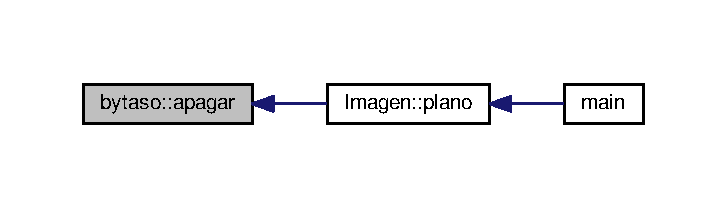
\includegraphics[width=349pt]{namespacebytaso_a29bc6fb2d3ca8a24ee9a8fc044aed54a_icgraph}
\end{center}
\end{figure}


\hypertarget{namespacebytaso_ae93ec524c1a740b4144a2ec249d07446}{}\index{bytaso@{bytaso}!asignar@{asignar}}
\index{asignar@{asignar}!bytaso@{bytaso}}
\subsubsection[{asignar(byte \&b, const bool v[])}]{\setlength{\rightskip}{0pt plus 5cm}void bytaso\+::asignar (
\begin{DoxyParamCaption}
\item[{{\bf byte} \&}]{b, }
\item[{const bool}]{v\mbox{[}$\,$\mbox{]}}
\end{DoxyParamCaption}
)}\label{namespacebytaso_ae93ec524c1a740b4144a2ec249d07446}


enciende los bits seg�n la configuraci�n de {\ttfamily v} 


\begin{DoxyParams}{Parámetros}
{\em b} & el {\ttfamily byte} sobre el que se quiere actuar \\
\hline
{\em v} & vector de 8 elementos que contiene la secuencia de bit\+S que se quieren asignar\\
\hline
\end{DoxyParams}
Asigna a {\ttfamily b} la configuraci�n de bits contenida en {\ttfamily v}. {\ttfamily v} es un vector de 8 booleanos donde {\ttfamily true} significa encendido y {\ttfamily false} significa apagado. \hypertarget{namespacebytaso_a01303edb3c075bbf9f10324914352a50}{}\index{bytaso@{bytaso}!byte\+To\+String@{byte\+To\+String}}
\index{byte\+To\+String@{byte\+To\+String}!bytaso@{bytaso}}
\subsubsection[{byte\+To\+String(byte b)}]{\setlength{\rightskip}{0pt plus 5cm}string bytaso\+::byte\+To\+String (
\begin{DoxyParamCaption}
\item[{{\bf byte}}]{b}
\end{DoxyParamCaption}
)}\label{namespacebytaso_a01303edb3c075bbf9f10324914352a50}


Muestra por la salida est�ndar una secuencia de 0s y 1s correspondiente al estado de cada bit. 


\begin{DoxyParams}{Parámetros}
{\em b} & el {\ttfamily byte} que se quiere imprimir\\
\hline
\end{DoxyParams}
Muestra por la salida est�ndar una secuencia de 0s y 1s correspondiente al estado de cada bit del byte donde un cero representa que un bit est� apagado y un uno que el bit est� encendido. Se implementa utilizando la funci�n \char`\"{}get\char`\"{}.

Por ejemplo, si en el {\ttfamily byte} {\ttfamily b} est�n encendidos los bits en posiciones 1 y 3 (0 m�s a la derecha), {\ttfamily print(b)}; mostrar� {\ttfamily 00001010} \hypertarget{namespacebytaso_a5e016205a37415abe06efd845593bc2a}{}\index{bytaso@{bytaso}!encender@{encender}}
\index{encender@{encender}!bytaso@{bytaso}}
\subsubsection[{encender(byte \&b)}]{\setlength{\rightskip}{0pt plus 5cm}void bytaso\+::encender (
\begin{DoxyParamCaption}
\item[{{\bf byte} \&}]{b}
\end{DoxyParamCaption}
)}\label{namespacebytaso_a5e016205a37415abe06efd845593bc2a}


enciende todos los bits 


\begin{DoxyParams}{Parámetros}
{\em b} & el {\ttfamily byte} que se quiere encender completamente. \\
\hline
\end{DoxyParams}
\hypertarget{namespacebytaso_a76ad23326440e16a7b419ee7a14ee287}{}\index{bytaso@{bytaso}!encendidos@{encendidos}}
\index{encendidos@{encendidos}!bytaso@{bytaso}}
\subsubsection[{encendidos(byte b, int posic[], int \&cuantos)}]{\setlength{\rightskip}{0pt plus 5cm}void bytaso\+::encendidos (
\begin{DoxyParamCaption}
\item[{{\bf byte}}]{b, }
\item[{int}]{posic\mbox{[}$\,$\mbox{]}, }
\item[{int \&}]{cuantos}
\end{DoxyParamCaption}
)}\label{namespacebytaso_a76ad23326440e16a7b419ee7a14ee287}


devuelve las posiciones de los bits encendidos 


\begin{DoxyParams}{Parámetros}
{\em b} & el {\ttfamily byte} que se quiere consultar \\
\hline
{\em posic} & vector de enteros (valores entre 0 a 7) que indican la posici�n de los bits de {\ttfamily b} que est�n encendidos \\
\hline
{\em cuantos} & n�mero de bits encendidos en {\ttfamily b} (n�mero de elementos usados en el vector {\ttfamily posic}) \\
\hline
\end{DoxyParams}


Gráfico de llamadas para esta función\+:
\nopagebreak
\begin{figure}[H]
\begin{center}
\leavevmode
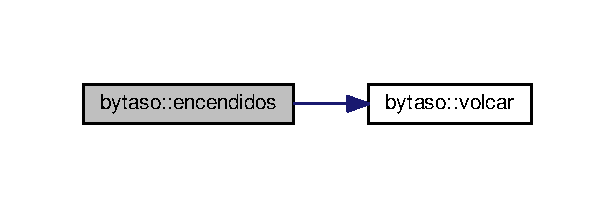
\includegraphics[width=295pt]{namespacebytaso_a76ad23326440e16a7b419ee7a14ee287_cgraph}
\end{center}
\end{figure}


\hypertarget{namespacebytaso_ad231ba96547f99130292527f5d65694b}{}\index{bytaso@{bytaso}!get@{get}}
\index{get@{get}!bytaso@{bytaso}}
\subsubsection[{get(byte b, int pos)}]{\setlength{\rightskip}{0pt plus 5cm}bool bytaso\+::get (
\begin{DoxyParamCaption}
\item[{{\bf byte}}]{b, }
\item[{int}]{pos}
\end{DoxyParamCaption}
)}\label{namespacebytaso_ad231ba96547f99130292527f5d65694b}


devuelve el estado del bit (encendido = true, apagado = false) en la posici�n {\ttfamily pos} 


\begin{DoxyParams}{Parámetros}
{\em b} & el {\ttfamily byte} que se quiere consultar \\
\hline
{\em pos} & el bit dentro de @ b que se quiere consultar (0 m�s a la derecha) \\
\hline
\end{DoxyParams}

\begin{DoxyRetVals}{Valores devueltos}
{\em true} & si el bit en la posici�n {\ttfamily pos} est� encendido \\
\hline
{\em false} & si el bit en la posici�n {\ttfamily pos} est� apagado \\
\hline
\end{DoxyRetVals}


Gráfico de llamadas a esta función\+:
\nopagebreak
\begin{figure}[H]
\begin{center}
\leavevmode
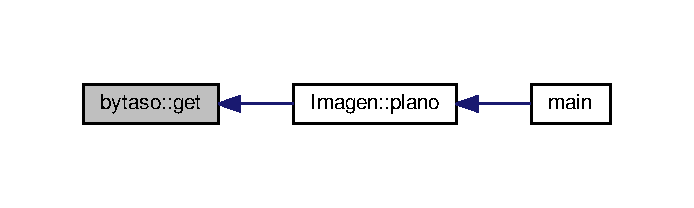
\includegraphics[width=333pt]{namespacebytaso_ad231ba96547f99130292527f5d65694b_icgraph}
\end{center}
\end{figure}


\hypertarget{namespacebytaso_a477a14f602dcc9264dbb6f874d170834}{}\index{bytaso@{bytaso}!off@{off}}
\index{off@{off}!bytaso@{bytaso}}
\subsubsection[{off(byte \&b, int pos)}]{\setlength{\rightskip}{0pt plus 5cm}void bytaso\+::off (
\begin{DoxyParamCaption}
\item[{{\bf byte} \&}]{b, }
\item[{int}]{pos}
\end{DoxyParamCaption}
)}\label{namespacebytaso_a477a14f602dcc9264dbb6f874d170834}


apaga el bit {\ttfamily pos} del {\ttfamily byte} {\ttfamily b} 


\begin{DoxyParams}{Parámetros}
{\em b} & el {\ttfamily byte} cuyo bit se quiere desactivar \\
\hline
{\em pos} & el bit dentro de {\ttfamily b} que se quiere desactivar (0 m�s a la derecha) \\
\hline
\end{DoxyParams}
\hypertarget{namespacebytaso_ae98a18093e63134e5f1ddec44973c6ec}{}\index{bytaso@{bytaso}!on@{on}}
\index{on@{on}!bytaso@{bytaso}}
\subsubsection[{on(byte \&b, int pos)}]{\setlength{\rightskip}{0pt plus 5cm}void bytaso\+::on (
\begin{DoxyParamCaption}
\item[{{\bf byte} \&}]{b, }
\item[{int}]{pos}
\end{DoxyParamCaption}
)}\label{namespacebytaso_ae98a18093e63134e5f1ddec44973c6ec}


enciende el bit {\ttfamily pos} del {\ttfamily byte} {\ttfamily b} 


\begin{DoxyParams}{Parámetros}
{\em b} & el {\ttfamily byte} cuyo bit se quiere activar \\
\hline
{\em pos} & el bit dentro de {\ttfamily b} que se quiere activar (0 m�s a la derecha) \\
\hline
\end{DoxyParams}


Gráfico de llamadas a esta función\+:
\nopagebreak
\begin{figure}[H]
\begin{center}
\leavevmode
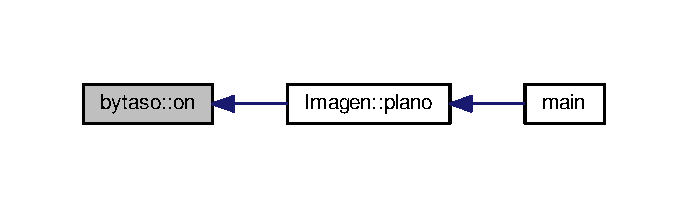
\includegraphics[width=330pt]{namespacebytaso_ae98a18093e63134e5f1ddec44973c6ec_icgraph}
\end{center}
\end{figure}


\hypertarget{namespacebytaso_aca892e499e255f8b8a967b67cd164a75}{}\index{bytaso@{bytaso}!volcar@{volcar}}
\index{volcar@{volcar}!bytaso@{bytaso}}
\subsubsection[{volcar(byte b, bool v[])}]{\setlength{\rightskip}{0pt plus 5cm}void bytaso\+::volcar (
\begin{DoxyParamCaption}
\item[{{\bf byte}}]{b, }
\item[{bool}]{v\mbox{[}$\,$\mbox{]}}
\end{DoxyParamCaption}
)}\label{namespacebytaso_aca892e499e255f8b8a967b67cd164a75}


recupera la configuraci�n de todos los bit 


\begin{DoxyParams}{Parámetros}
{\em b} & el {\ttfamily byte} que se quiere consultar \\
\hline
{\em v} & vector de 8 elementos que contendr� el estado de cada uno de los bits de @ b\\
\hline
\end{DoxyParams}
Vuelca en {\ttfamily v} la configuraci�n de bits contenida en {\ttfamily b}. {\ttfamily true} significa encendido y {\ttfamily false} significa apagado. El tama�o de {\ttfamily v} debe ser 8. 

Gráfico de llamadas a esta función\+:
\nopagebreak
\begin{figure}[H]
\begin{center}
\leavevmode
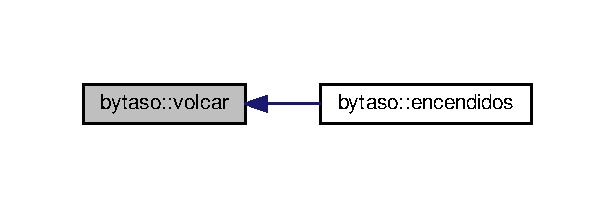
\includegraphics[width=295pt]{namespacebytaso_aca892e499e255f8b8a967b67cd164a75_icgraph}
\end{center}
\end{figure}



\chapter{Documentación de las clases}
\hypertarget{struct_celda}{}\section{Referencia de la Estructura Celda}
\label{struct_celda}\index{Celda@{Celda}}


{\ttfamily \#include $<$lista.\+h$>$}



Diagrama de colaboración para Celda\+:
\nopagebreak
\begin{figure}[H]
\begin{center}
\leavevmode
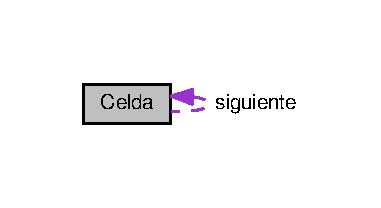
\includegraphics[width=183pt]{struct_celda__coll__graph}
\end{center}
\end{figure}
\subsection*{Atributos públicos}
\begin{DoxyCompactItemize}
\item 
string \hyperlink{struct_celda_aef12ed8e6d15d140a516c259cdcbf634}{datos}
\item 
\hyperlink{struct_celda}{Celda} $\ast$ \hyperlink{struct_celda_a5c6d6d20b0c0b0a359715844955a0078}{siguiente}
\begin{DoxyCompactList}\small\item\em valor de la celda actual \end{DoxyCompactList}\end{DoxyCompactItemize}


\subsection{Documentación de los datos miembro}
\hypertarget{struct_celda_aef12ed8e6d15d140a516c259cdcbf634}{}\index{Celda@{Celda}!datos@{datos}}
\index{datos@{datos}!Celda@{Celda}}
\subsubsection[{datos}]{\setlength{\rightskip}{0pt plus 5cm}string Celda\+::datos}\label{struct_celda_aef12ed8e6d15d140a516c259cdcbf634}
\hypertarget{struct_celda_a5c6d6d20b0c0b0a359715844955a0078}{}\index{Celda@{Celda}!siguiente@{siguiente}}
\index{siguiente@{siguiente}!Celda@{Celda}}
\subsubsection[{siguiente}]{\setlength{\rightskip}{0pt plus 5cm}{\bf Celda}$\ast$ Celda\+::siguiente}\label{struct_celda_a5c6d6d20b0c0b0a359715844955a0078}


valor de la celda actual 



La documentación para esta estructura fue generada a partir del siguiente fichero\+:\begin{DoxyCompactItemize}
\item 
include/\hyperlink{lista_8h}{lista.\+h}\end{DoxyCompactItemize}

\hypertarget{class_imagen}{}\section{Referencia de la Clase Imagen}
\label{class_imagen}\index{Imagen@{Imagen}}


Una imagen en blanco y negro. Cada píxel es un byte.  




{\ttfamily \#include $<$imagen.\+h$>$}

\subsection*{Métodos públicos}
\begin{DoxyCompactItemize}
\item 
\hyperlink{class_imagen_ab2e649aa7a105155c7bfdb846abf0528}{Imagen} ()
\begin{DoxyCompactList}\small\item\em Constructor por defecto. Crea un \hyperlink{class_imagen}{Imagen} vacía de 0 filas x 0 columnas. \end{DoxyCompactList}\item 
\hyperlink{class_imagen_a03dd93c9cf920a9dc0b72f8bd34f2e8a}{$\sim$\+Imagen} ()
\begin{DoxyCompactList}\small\item\em Libera la memoria reservada para una imagen. \end{DoxyCompactList}\item 
\hyperlink{class_imagen_ac21b1c758a32e6c43315b9f46caf673e}{Imagen} (const \hyperlink{class_imagen}{Imagen} \&)
\begin{DoxyCompactList}\small\item\em Contructor de copia de la clase \hyperlink{class_imagen}{Imagen}. \end{DoxyCompactList}\item 
\hyperlink{class_imagen}{Imagen} \& \hyperlink{class_imagen_a43d10ec74966d22e5477f686462802dc}{operator=} (const \hyperlink{class_imagen}{Imagen} \&img)
\begin{DoxyCompactList}\small\item\em Operador de asignación de la clase imagen. Si la imagen a asignar es la misma que la actual no hace nada. Si la imagen ya estaba creada, se destruye. \end{DoxyCompactList}\item 
\hyperlink{class_imagen}{Imagen} \hyperlink{class_imagen_afc8f4a032d37f2012f1175599f81d60b}{operator+} (\hyperlink{class_imagen}{Imagen} img)
\begin{DoxyCompactList}\small\item\em Operador + de la clase imagen. Devuelve una nueva imagen compuesta por los dos sumandos colocados uno al lado del otro y con el espacio que quede en negro. \end{DoxyCompactList}\item 
\hyperlink{class_imagen_a7632978f5ae089713e652bb362da1e78}{Imagen} (int \hyperlink{class_imagen_af74657d5c16a52feeda9d233cfe29b33}{filas}, int \hyperlink{class_imagen_aaed2f76db10125985aac80e439ec7b6d}{columnas})
\begin{DoxyCompactList}\small\item\em Construye una imagen negra de tamaño {\itshape filas} x {\itshape columnas}. \end{DoxyCompactList}\item 
void \hyperlink{class_imagen_a3c963c0aaa02767f65b4510cb39027ac}{crear} (int \hyperlink{class_imagen_af74657d5c16a52feeda9d233cfe29b33}{filas}, int \hyperlink{class_imagen_aaed2f76db10125985aac80e439ec7b6d}{columnas})
\begin{DoxyCompactList}\small\item\em Crea una imagen negra de tamaño {\itshape filas} x {\itshape columnas}. \end{DoxyCompactList}\item 
int \hyperlink{class_imagen_af74657d5c16a52feeda9d233cfe29b33}{filas} () const 
\begin{DoxyCompactList}\small\item\em Devuelve el número de filas de las imagen. \end{DoxyCompactList}\item 
int \hyperlink{class_imagen_aaed2f76db10125985aac80e439ec7b6d}{columnas} () const 
\begin{DoxyCompactList}\small\item\em Devuelve el número de columnas de las imagen. \end{DoxyCompactList}\item 
void \hyperlink{class_imagen_a722347f0110d794f96c92beda6710158}{set} (int y, int x, \hyperlink{imagen_8h_a0c8186d9b9b7880309c27230bbb5e69d}{byte} v)
\begin{DoxyCompactList}\small\item\em Asigna el valor {\itshape v} a la posición ({\itshape x},{\itshape y}) de la imagen. \end{DoxyCompactList}\item 
\hyperlink{imagen_8h_a0c8186d9b9b7880309c27230bbb5e69d}{byte} \hyperlink{class_imagen_ab8a0d7d44f6d22678ed7fea1e9617e25}{get} (int y, int x)
\begin{DoxyCompactList}\small\item\em Devuelve el valor de la posición ({\itshape x},{\itshape y}) de la imagen. \end{DoxyCompactList}\item 
void \hyperlink{class_imagen_a9c1bfd9bff6ae8851f3e0c9ac2e90382}{set\+Pos} (int i, \hyperlink{imagen_8h_a0c8186d9b9b7880309c27230bbb5e69d}{byte} v)
\begin{DoxyCompactList}\small\item\em Asigna el valor {\itshape v} a la posición {\itshape i} de la imagen considerada como vector. \end{DoxyCompactList}\item 
\hyperlink{imagen_8h_a0c8186d9b9b7880309c27230bbb5e69d}{byte} \hyperlink{class_imagen_a00b702abaaf3261ade141597beb7bc55}{get\+Pos} (int i) const 
\begin{DoxyCompactList}\small\item\em Devuelve el valor de la posición {\itshape i} de la imagen considerada como vector. \end{DoxyCompactList}\item 
bool \hyperlink{class_imagen_aa46cc99da218afa01f55395e4c96ffe0}{leer\+Imagen} (const char nombre\+Fichero\mbox{[}$\,$\mbox{]})
\begin{DoxyCompactList}\small\item\em Carga una imagen desde un fichero. \end{DoxyCompactList}\item 
bool \hyperlink{class_imagen_aec07c487f3cb1ea1fdd26cb555f02ed1}{escribir\+Imagen} (const char nombre\+Fichero\mbox{[}$\,$\mbox{]}, bool es\+Binario)
\begin{DoxyCompactList}\small\item\em Guarda una imagen desde un fichero. \end{DoxyCompactList}\item 
\hyperlink{class_imagen}{Imagen} $\ast$ \hyperlink{class_imagen_a738d3b88a80606af9d78458e5586e04c}{plano} (int k)
\begin{DoxyCompactList}\small\item\em Extrae de la imagen el plano del bit del vector indicado por {\itshape k}. \end{DoxyCompactList}\item 
bool \hyperlink{class_imagen_aa5c1f94763ca1774792548daa3d0e793}{a\+Arte\+A\+S\+C\+I\+I} (const char grises\mbox{[}$\,$\mbox{]}, char arte\+A\+S\+C\+I\+I\mbox{[}$\,$\mbox{]}, int maxlong)
\begin{DoxyCompactList}\small\item\em Dada una imagen, se convierte equivalente utilizando caracteres A\+S\+C\+I\+I. \end{DoxyCompactList}\item 
bool \hyperlink{class_imagen_a0266a25af1413cb57d9da880e7881860}{lista\+A\+Arte\+A\+S\+C\+I\+I} (const \hyperlink{class_lista}{Lista} \&celdas)
\begin{DoxyCompactList}\small\item\em Dada una lista de strings que representan niveles de gris, se ejecuta la función  a\+Arte\+A\+S\+C\+I\+I con cada string. El resultado de pasar la imagen a arte A\+S\+C\+I\+I con cada grupo de grises se guarda en archivos con nombre ascii1.\+txt, ascii2.\+txt,... \end{DoxyCompactList}\item 
void \hyperlink{class_imagen_aea77aed960516bf385f94249f074dd9a}{destruir} ()
\begin{DoxyCompactList}\small\item\em Libera la memoria de una imagen. Esta función es llamada por el destructor. \end{DoxyCompactList}\end{DoxyCompactItemize}
\subsection*{Atributos privados}
\begin{DoxyCompactItemize}
\item 
\hyperlink{imagen_8h_a0c8186d9b9b7880309c27230bbb5e69d}{byte} $\ast$$\ast$ \hyperlink{class_imagen_a74bf3487e42bb65862e994883fa05b33}{datos}
\begin{DoxyCompactList}\small\item\em puntero a los punteros de las filas \end{DoxyCompactList}\item 
int \hyperlink{class_imagen_a89599a9692fbe4cb60ee16c0a30a64ef}{nfilas}
\begin{DoxyCompactList}\small\item\em número de filas de la imagen \end{DoxyCompactList}\item 
int \hyperlink{class_imagen_a4b38c0642ab84fe5f945272180ae8306}{ncolumnas}
\begin{DoxyCompactList}\small\item\em número de columnsa de la imagen \end{DoxyCompactList}\end{DoxyCompactItemize}


\subsection{Descripción detallada}
Una imagen en blanco y negro. Cada píxel es un byte. 

\subsection{Documentación del constructor y destructor}
\hypertarget{class_imagen_ab2e649aa7a105155c7bfdb846abf0528}{}\index{Imagen@{Imagen}!Imagen@{Imagen}}
\index{Imagen@{Imagen}!Imagen@{Imagen}}
\subsubsection[{Imagen()}]{\setlength{\rightskip}{0pt plus 5cm}Imagen\+::\+Imagen (
\begin{DoxyParamCaption}
{}
\end{DoxyParamCaption}
)}\label{class_imagen_ab2e649aa7a105155c7bfdb846abf0528}


Constructor por defecto. Crea un \hyperlink{class_imagen}{Imagen} vacía de 0 filas x 0 columnas. 

\hypertarget{class_imagen_a03dd93c9cf920a9dc0b72f8bd34f2e8a}{}\index{Imagen@{Imagen}!````~Imagen@{$\sim$\+Imagen}}
\index{````~Imagen@{$\sim$\+Imagen}!Imagen@{Imagen}}
\subsubsection[{$\sim$\+Imagen()}]{\setlength{\rightskip}{0pt plus 5cm}Imagen\+::$\sim$\+Imagen (
\begin{DoxyParamCaption}
{}
\end{DoxyParamCaption}
)}\label{class_imagen_a03dd93c9cf920a9dc0b72f8bd34f2e8a}


Libera la memoria reservada para una imagen. 

\hypertarget{class_imagen_ac21b1c758a32e6c43315b9f46caf673e}{}\index{Imagen@{Imagen}!Imagen@{Imagen}}
\index{Imagen@{Imagen}!Imagen@{Imagen}}
\subsubsection[{Imagen(const Imagen \&)}]{\setlength{\rightskip}{0pt plus 5cm}Imagen\+::\+Imagen (
\begin{DoxyParamCaption}
\item[{const {\bf Imagen} \&}]{img}
\end{DoxyParamCaption}
)}\label{class_imagen_ac21b1c758a32e6c43315b9f46caf673e}


Contructor de copia de la clase \hyperlink{class_imagen}{Imagen}. 


\begin{DoxyParams}{Parámetros}
{\em \hyperlink{class_imagen}{Imagen}} & a copiar \\
\hline
\end{DoxyParams}


Gráfico de llamadas para esta función\+:
\nopagebreak
\begin{figure}[H]
\begin{center}
\leavevmode
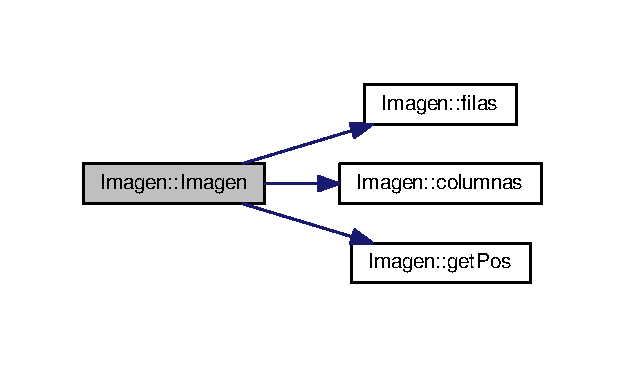
\includegraphics[width=300pt]{class_imagen_ac21b1c758a32e6c43315b9f46caf673e_cgraph}
\end{center}
\end{figure}


\hypertarget{class_imagen_a7632978f5ae089713e652bb362da1e78}{}\index{Imagen@{Imagen}!Imagen@{Imagen}}
\index{Imagen@{Imagen}!Imagen@{Imagen}}
\subsubsection[{Imagen(int filas, int columnas)}]{\setlength{\rightskip}{0pt plus 5cm}Imagen\+::\+Imagen (
\begin{DoxyParamCaption}
\item[{int}]{filas, }
\item[{int}]{columnas}
\end{DoxyParamCaption}
)}\label{class_imagen_a7632978f5ae089713e652bb362da1e78}


Construye una imagen negra de tamaño {\itshape filas} x {\itshape columnas}. 


\begin{DoxyParams}{Parámetros}
{\em filas} & número de filas de la imagen \\
\hline
{\em columnas} & número de columnas de la imagen\\
\hline
\end{DoxyParams}
Construye una imagen de tamaño {\itshape filas} x {\itshape columnas} y pone todos sus elementos a 0. 

\subsection{Documentación de las funciones miembro}
\hypertarget{class_imagen_aa5c1f94763ca1774792548daa3d0e793}{}\index{Imagen@{Imagen}!a\+Arte\+A\+S\+C\+I\+I@{a\+Arte\+A\+S\+C\+I\+I}}
\index{a\+Arte\+A\+S\+C\+I\+I@{a\+Arte\+A\+S\+C\+I\+I}!Imagen@{Imagen}}
\subsubsection[{a\+Arte\+A\+S\+C\+I\+I(const char grises[], char arte\+A\+S\+C\+I\+I[], int maxlong)}]{\setlength{\rightskip}{0pt plus 5cm}bool Imagen\+::a\+Arte\+A\+S\+C\+I\+I (
\begin{DoxyParamCaption}
\item[{const char}]{grises\mbox{[}$\,$\mbox{]}, }
\item[{char}]{arte\+A\+S\+C\+I\+I\mbox{[}$\,$\mbox{]}, }
\item[{int}]{maxlong}
\end{DoxyParamCaption}
)}\label{class_imagen_aa5c1f94763ca1774792548daa3d0e793}


Dada una imagen, se convierte equivalente utilizando caracteres A\+S\+C\+I\+I. 


\begin{DoxyParams}{Parámetros}
{\em grises} & caracteres que se utilizarán en el arte A\+S\+C\+I\+I \\
\hline
{\em arte\+A\+S\+C\+I\+I} & vector resultante con la cadena A\+S\+C\+I\+I que representa la imagen \\
\hline
{\em maxlong} & longitud máxima \\
\hline
\end{DoxyParams}

\begin{DoxyRetVals}{Valores devueltos}
{\em true} & la imagen cabe en el vector resultante \\
\hline
{\em false} & la imagen no cabe en el vector resultante \\
\hline
\end{DoxyRetVals}


Gráfico de llamadas a esta función\+:
\nopagebreak
\begin{figure}[H]
\begin{center}
\leavevmode
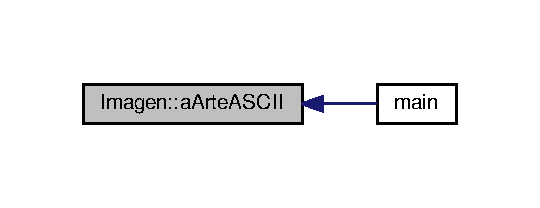
\includegraphics[width=259pt]{class_imagen_aa5c1f94763ca1774792548daa3d0e793_icgraph}
\end{center}
\end{figure}


\hypertarget{class_imagen_aaed2f76db10125985aac80e439ec7b6d}{}\index{Imagen@{Imagen}!columnas@{columnas}}
\index{columnas@{columnas}!Imagen@{Imagen}}
\subsubsection[{columnas() const }]{\setlength{\rightskip}{0pt plus 5cm}int Imagen\+::columnas (
\begin{DoxyParamCaption}
{}
\end{DoxyParamCaption}
) const}\label{class_imagen_aaed2f76db10125985aac80e439ec7b6d}


Devuelve el número de columnas de las imagen. 

\begin{DoxyReturn}{Devuelve}
el número de columnas de la imagen 
\end{DoxyReturn}


Gráfico de llamadas a esta función\+:
\nopagebreak
\begin{figure}[H]
\begin{center}
\leavevmode
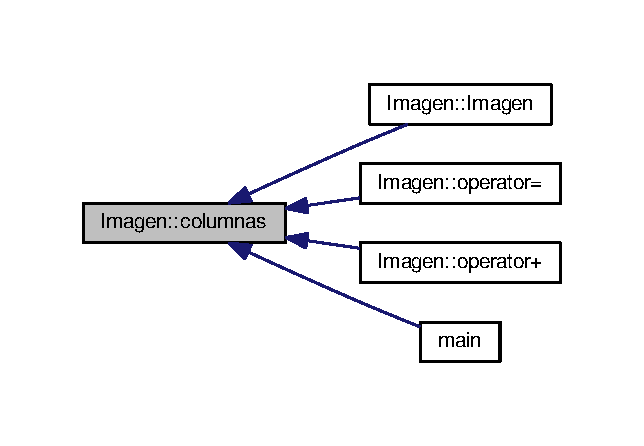
\includegraphics[width=309pt]{class_imagen_aaed2f76db10125985aac80e439ec7b6d_icgraph}
\end{center}
\end{figure}


\hypertarget{class_imagen_a3c963c0aaa02767f65b4510cb39027ac}{}\index{Imagen@{Imagen}!crear@{crear}}
\index{crear@{crear}!Imagen@{Imagen}}
\subsubsection[{crear(int filas, int columnas)}]{\setlength{\rightskip}{0pt plus 5cm}void Imagen\+::crear (
\begin{DoxyParamCaption}
\item[{int}]{filas, }
\item[{int}]{columnas}
\end{DoxyParamCaption}
)}\label{class_imagen_a3c963c0aaa02767f65b4510cb39027ac}


Crea una imagen negra de tamaño {\itshape filas} x {\itshape columnas}. 


\begin{DoxyParams}{Parámetros}
{\em filas} & número de filas de la imagen \\
\hline
{\em columnas} & número de columnas de la imagen\\
\hline
\end{DoxyParams}
Dimensiona la imagen a tamaño {\itshape filas} x {\itshape columnas} y pone todos sus elementos a 0. 

Gráfico de llamadas a esta función\+:
\nopagebreak
\begin{figure}[H]
\begin{center}
\leavevmode
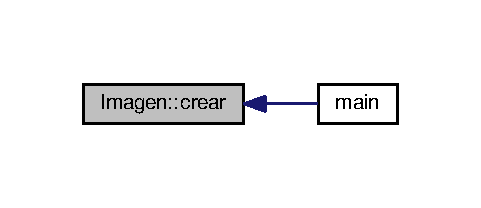
\includegraphics[width=231pt]{class_imagen_a3c963c0aaa02767f65b4510cb39027ac_icgraph}
\end{center}
\end{figure}


\hypertarget{class_imagen_aea77aed960516bf385f94249f074dd9a}{}\index{Imagen@{Imagen}!destruir@{destruir}}
\index{destruir@{destruir}!Imagen@{Imagen}}
\subsubsection[{destruir()}]{\setlength{\rightskip}{0pt plus 5cm}void Imagen\+::destruir (
\begin{DoxyParamCaption}
{}
\end{DoxyParamCaption}
)}\label{class_imagen_aea77aed960516bf385f94249f074dd9a}


Libera la memoria de una imagen. Esta función es llamada por el destructor. 



Gráfico de llamadas a esta función\+:
\nopagebreak
\begin{figure}[H]
\begin{center}
\leavevmode
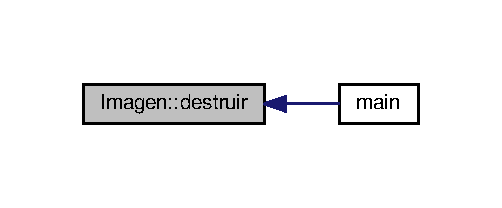
\includegraphics[width=241pt]{class_imagen_aea77aed960516bf385f94249f074dd9a_icgraph}
\end{center}
\end{figure}


\hypertarget{class_imagen_aec07c487f3cb1ea1fdd26cb555f02ed1}{}\index{Imagen@{Imagen}!escribir\+Imagen@{escribir\+Imagen}}
\index{escribir\+Imagen@{escribir\+Imagen}!Imagen@{Imagen}}
\subsubsection[{escribir\+Imagen(const char nombre\+Fichero[], bool es\+Binario)}]{\setlength{\rightskip}{0pt plus 5cm}bool Imagen\+::escribir\+Imagen (
\begin{DoxyParamCaption}
\item[{const char}]{nombre\+Fichero\mbox{[}$\,$\mbox{]}, }
\item[{bool}]{es\+Binario}
\end{DoxyParamCaption}
)}\label{class_imagen_aec07c487f3cb1ea1fdd26cb555f02ed1}


Guarda una imagen desde un fichero. 


\begin{DoxyParams}{Parámetros}
{\em nombre\+Fichero} & nombre del fichero que contiene la imagen \\
\hline
{\em es\+Binario} & toma el valor {\ttfamily true} si el fichero se escribe en formato binario o {\ttfamily false} en caso contrario. \\
\hline
\end{DoxyParams}

\begin{DoxyRetVals}{Valores devueltos}
{\em true} & si ha tenido éxito en la escritura \\
\hline
{\em false} & si se ha producido algún error en la escritura \\
\hline
\end{DoxyRetVals}


Gráfico de llamadas para esta función\+:
\nopagebreak
\begin{figure}[H]
\begin{center}
\leavevmode
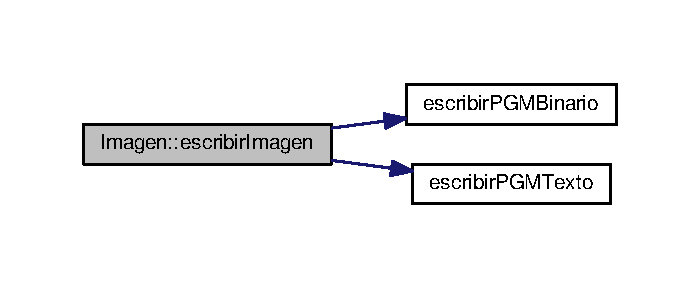
\includegraphics[width=336pt]{class_imagen_aec07c487f3cb1ea1fdd26cb555f02ed1_cgraph}
\end{center}
\end{figure}




Gráfico de llamadas a esta función\+:
\nopagebreak
\begin{figure}[H]
\begin{center}
\leavevmode
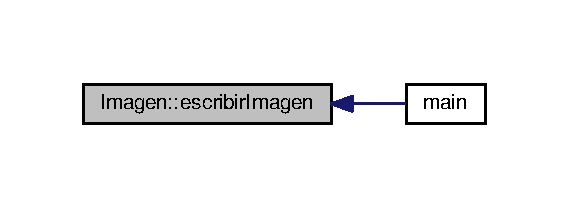
\includegraphics[width=273pt]{class_imagen_aec07c487f3cb1ea1fdd26cb555f02ed1_icgraph}
\end{center}
\end{figure}


\hypertarget{class_imagen_af74657d5c16a52feeda9d233cfe29b33}{}\index{Imagen@{Imagen}!filas@{filas}}
\index{filas@{filas}!Imagen@{Imagen}}
\subsubsection[{filas() const }]{\setlength{\rightskip}{0pt plus 5cm}int Imagen\+::filas (
\begin{DoxyParamCaption}
{}
\end{DoxyParamCaption}
) const}\label{class_imagen_af74657d5c16a52feeda9d233cfe29b33}


Devuelve el número de filas de las imagen. 

\begin{DoxyReturn}{Devuelve}
el número de filas de la imagen 
\end{DoxyReturn}


Gráfico de llamadas a esta función\+:
\nopagebreak
\begin{figure}[H]
\begin{center}
\leavevmode
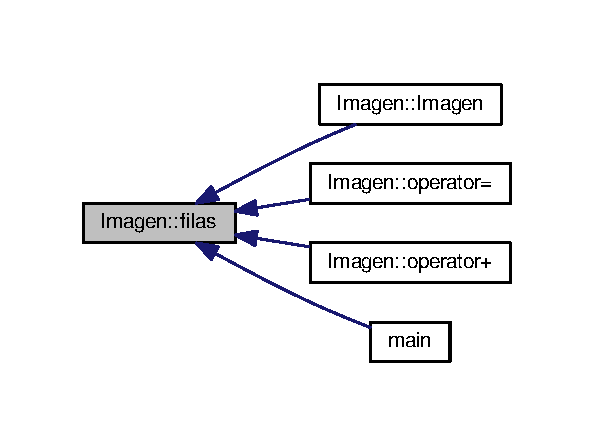
\includegraphics[width=285pt]{class_imagen_af74657d5c16a52feeda9d233cfe29b33_icgraph}
\end{center}
\end{figure}


\hypertarget{class_imagen_ab8a0d7d44f6d22678ed7fea1e9617e25}{}\index{Imagen@{Imagen}!get@{get}}
\index{get@{get}!Imagen@{Imagen}}
\subsubsection[{get(int y, int x)}]{\setlength{\rightskip}{0pt plus 5cm}{\bf byte} Imagen\+::get (
\begin{DoxyParamCaption}
\item[{int}]{y, }
\item[{int}]{x}
\end{DoxyParamCaption}
)}\label{class_imagen_ab8a0d7d44f6d22678ed7fea1e9617e25}


Devuelve el valor de la posición ({\itshape x},{\itshape y}) de la imagen. 


\begin{DoxyParams}{Parámetros}
{\em y} & fila de la imagen \\
\hline
{\em x} & columna de la imagen \\
\hline
\end{DoxyParams}
\begin{DoxyReturn}{Devuelve}
el valor de la posición ({\itshape x},{\itshape y}) de la imagen
\end{DoxyReturn}
Devuelve el valor de la posición ({\itshape x},{\itshape y}) de la imagen. Dado que la imagen se guarda como un vector, la posición ({\itshape x},{\itshape y}) corresponde a la posición {\itshape y} $\ast$ {\ttfamily ncolumnas} + {\itshape x} del vector. 

Gráfico de llamadas a esta función\+:
\nopagebreak
\begin{figure}[H]
\begin{center}
\leavevmode
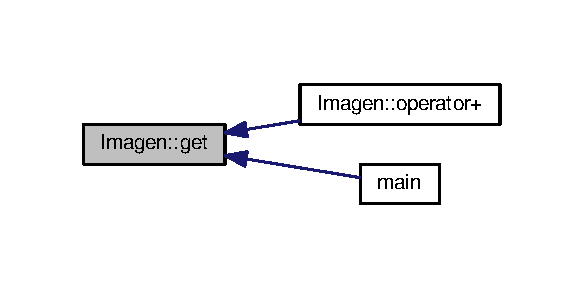
\includegraphics[width=280pt]{class_imagen_ab8a0d7d44f6d22678ed7fea1e9617e25_icgraph}
\end{center}
\end{figure}


\hypertarget{class_imagen_a00b702abaaf3261ade141597beb7bc55}{}\index{Imagen@{Imagen}!get\+Pos@{get\+Pos}}
\index{get\+Pos@{get\+Pos}!Imagen@{Imagen}}
\subsubsection[{get\+Pos(int i) const }]{\setlength{\rightskip}{0pt plus 5cm}{\bf byte} Imagen\+::get\+Pos (
\begin{DoxyParamCaption}
\item[{int}]{i}
\end{DoxyParamCaption}
) const}\label{class_imagen_a00b702abaaf3261ade141597beb7bc55}


Devuelve el valor de la posición {\itshape i} de la imagen considerada como vector. 


\begin{DoxyParams}{Parámetros}
{\em i} & posición de la imagen considerada como vector\\
\hline
\end{DoxyParams}
Devuelve el valor de la posición {\itshape i} de la imagen considerada como vector. La posición {\itshape i} corresponde con la posición {\ttfamily y} $\ast$ {\ttfamily ncolumnas} + {\ttfamily x} de la imagen donde {\ttfamily y} representa la fila y {\ttfamily x} representa la columna. 

Gráfico de llamadas a esta función\+:
\nopagebreak
\begin{figure}[H]
\begin{center}
\leavevmode
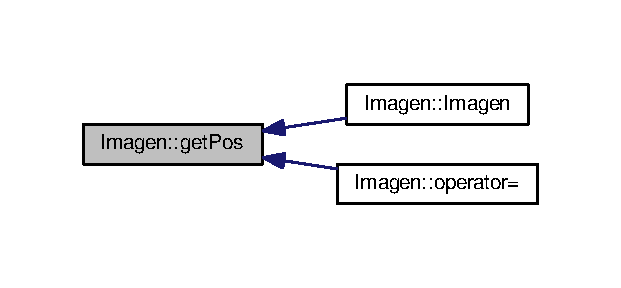
\includegraphics[width=298pt]{class_imagen_a00b702abaaf3261ade141597beb7bc55_icgraph}
\end{center}
\end{figure}


\hypertarget{class_imagen_aa46cc99da218afa01f55395e4c96ffe0}{}\index{Imagen@{Imagen}!leer\+Imagen@{leer\+Imagen}}
\index{leer\+Imagen@{leer\+Imagen}!Imagen@{Imagen}}
\subsubsection[{leer\+Imagen(const char nombre\+Fichero[])}]{\setlength{\rightskip}{0pt plus 5cm}bool Imagen\+::leer\+Imagen (
\begin{DoxyParamCaption}
\item[{const char}]{nombre\+Fichero\mbox{[}$\,$\mbox{]}}
\end{DoxyParamCaption}
)}\label{class_imagen_aa46cc99da218afa01f55395e4c96ffe0}


Carga una imagen desde un fichero. 


\begin{DoxyParams}{Parámetros}
{\em nombre\+Fichero} & nombre del fichero que contiene la imagen \\
\hline
\end{DoxyParams}

\begin{DoxyRetVals}{Valores devueltos}
{\em true} & si ha tenido éxito en la lectura \\
\hline
{\em false} & si se ha producido algún error en la lectura\\
\hline
\end{DoxyRetVals}
Lee desde disco los datos de la imagen llamada {\itshape nombre\+Fichero} y la guarda en la memoria. La función debe asegurarse de que la imagen es de un tipo de imagen conocido. 

Gráfico de llamadas para esta función\+:
\nopagebreak
\begin{figure}[H]
\begin{center}
\leavevmode
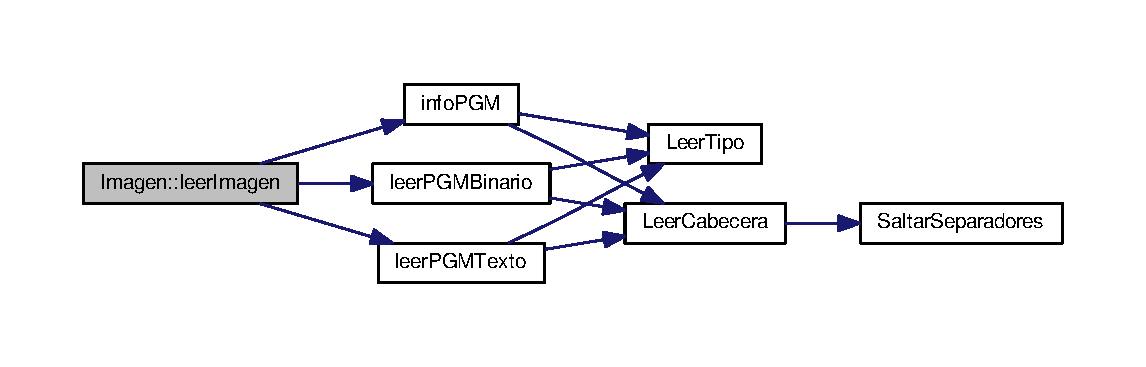
\includegraphics[width=350pt]{class_imagen_aa46cc99da218afa01f55395e4c96ffe0_cgraph}
\end{center}
\end{figure}




Gráfico de llamadas a esta función\+:
\nopagebreak
\begin{figure}[H]
\begin{center}
\leavevmode
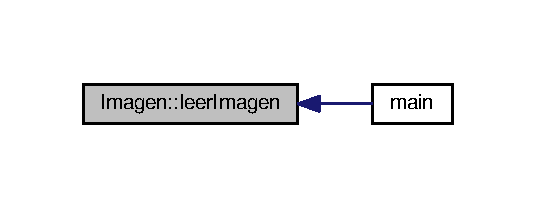
\includegraphics[width=257pt]{class_imagen_aa46cc99da218afa01f55395e4c96ffe0_icgraph}
\end{center}
\end{figure}


\hypertarget{class_imagen_a0266a25af1413cb57d9da880e7881860}{}\index{Imagen@{Imagen}!lista\+A\+Arte\+A\+S\+C\+I\+I@{lista\+A\+Arte\+A\+S\+C\+I\+I}}
\index{lista\+A\+Arte\+A\+S\+C\+I\+I@{lista\+A\+Arte\+A\+S\+C\+I\+I}!Imagen@{Imagen}}
\subsubsection[{lista\+A\+Arte\+A\+S\+C\+I\+I(const Lista \&celdas)}]{\setlength{\rightskip}{0pt plus 5cm}bool Imagen\+::lista\+A\+Arte\+A\+S\+C\+I\+I (
\begin{DoxyParamCaption}
\item[{const {\bf Lista} \&}]{celdas}
\end{DoxyParamCaption}
)}\label{class_imagen_a0266a25af1413cb57d9da880e7881860}


Dada una lista de strings que representan niveles de gris, se ejecuta la función  a\+Arte\+A\+S\+C\+I\+I con cada string. El resultado de pasar la imagen a arte A\+S\+C\+I\+I con cada grupo de grises se guarda en archivos con nombre ascii1.\+txt, ascii2.\+txt,... 


\begin{DoxyParams}{Parámetros}
{\em celdas} & \hyperlink{class_lista}{Lista} de strings de niveles de gris \\
\hline
\end{DoxyParams}

\begin{DoxyRetVals}{Valores devueltos}
{\em true} & todas las conversiones fueron posibles \\
\hline
{\em false} & alguna conversión falló \\
\hline
\end{DoxyRetVals}


Gráfico de llamadas para esta función\+:
\nopagebreak
\begin{figure}[H]
\begin{center}
\leavevmode
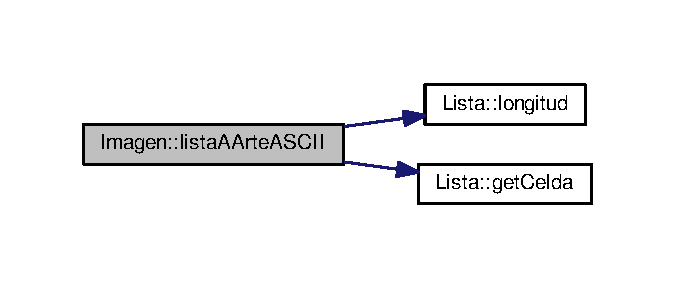
\includegraphics[width=324pt]{class_imagen_a0266a25af1413cb57d9da880e7881860_cgraph}
\end{center}
\end{figure}




Gráfico de llamadas a esta función\+:
\nopagebreak
\begin{figure}[H]
\begin{center}
\leavevmode
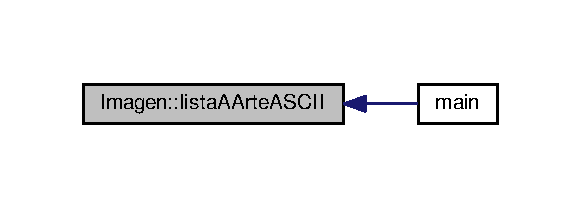
\includegraphics[width=279pt]{class_imagen_a0266a25af1413cb57d9da880e7881860_icgraph}
\end{center}
\end{figure}


\hypertarget{class_imagen_afc8f4a032d37f2012f1175599f81d60b}{}\index{Imagen@{Imagen}!operator+@{operator+}}
\index{operator+@{operator+}!Imagen@{Imagen}}
\subsubsection[{operator+(\+Imagen img)}]{\setlength{\rightskip}{0pt plus 5cm}{\bf Imagen} Imagen\+::operator+ (
\begin{DoxyParamCaption}
\item[{{\bf Imagen}}]{img}
\end{DoxyParamCaption}
)}\label{class_imagen_afc8f4a032d37f2012f1175599f81d60b}


Operador + de la clase imagen. Devuelve una nueva imagen compuesta por los dos sumandos colocados uno al lado del otro y con el espacio que quede en negro. 


\begin{DoxyParams}{Parámetros}
{\em img} & imagen a sumar \\
\hline
\end{DoxyParams}
\begin{DoxyReturn}{Devuelve}
imagen suma 
\end{DoxyReturn}


Gráfico de llamadas para esta función\+:
\nopagebreak
\begin{figure}[H]
\begin{center}
\leavevmode
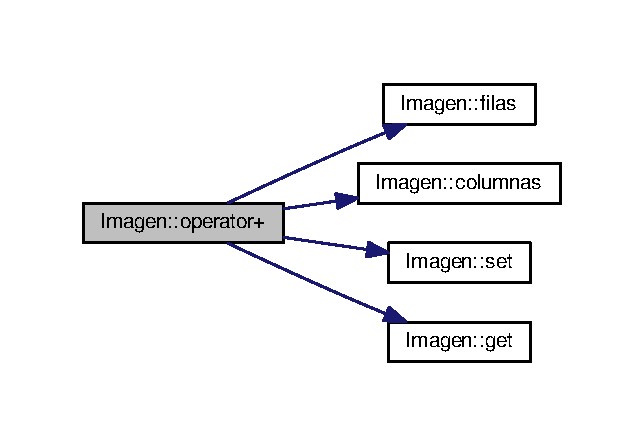
\includegraphics[width=309pt]{class_imagen_afc8f4a032d37f2012f1175599f81d60b_cgraph}
\end{center}
\end{figure}


\hypertarget{class_imagen_a43d10ec74966d22e5477f686462802dc}{}\index{Imagen@{Imagen}!operator=@{operator=}}
\index{operator=@{operator=}!Imagen@{Imagen}}
\subsubsection[{operator=(const Imagen \&img)}]{\setlength{\rightskip}{0pt plus 5cm}{\bf Imagen} \& Imagen\+::operator= (
\begin{DoxyParamCaption}
\item[{const {\bf Imagen} \&}]{img}
\end{DoxyParamCaption}
)}\label{class_imagen_a43d10ec74966d22e5477f686462802dc}


Operador de asignación de la clase imagen. Si la imagen a asignar es la misma que la actual no hace nada. Si la imagen ya estaba creada, se destruye. 


\begin{DoxyParams}{Parámetros}
{\em img} & imagen a copiar \\
\hline
\end{DoxyParams}
\begin{DoxyReturn}{Devuelve}
imagen nueva copiada 
\end{DoxyReturn}


Gráfico de llamadas para esta función\+:
\nopagebreak
\begin{figure}[H]
\begin{center}
\leavevmode
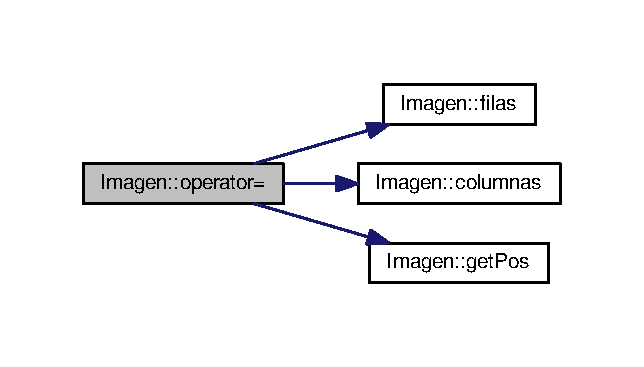
\includegraphics[width=309pt]{class_imagen_a43d10ec74966d22e5477f686462802dc_cgraph}
\end{center}
\end{figure}


\hypertarget{class_imagen_a738d3b88a80606af9d78458e5586e04c}{}\index{Imagen@{Imagen}!plano@{plano}}
\index{plano@{plano}!Imagen@{Imagen}}
\subsubsection[{plano(int k)}]{\setlength{\rightskip}{0pt plus 5cm}{\bf Imagen} $\ast$ Imagen\+::plano (
\begin{DoxyParamCaption}
\item[{int}]{k}
\end{DoxyParamCaption}
)}\label{class_imagen_a738d3b88a80606af9d78458e5586e04c}


Extrae de la imagen el plano del bit del vector indicado por {\itshape k}. 


\begin{DoxyParams}{Parámetros}
{\em k} & Numero del bit del que extraer el plano\\
\hline
\end{DoxyParams}
Extrae de la imagen el plano de la imagen del bit indicado por {\itshape k}, despues devuelve como una nueva imagen el plano resultante. 

Gráfico de llamadas para esta función\+:
\nopagebreak
\begin{figure}[H]
\begin{center}
\leavevmode
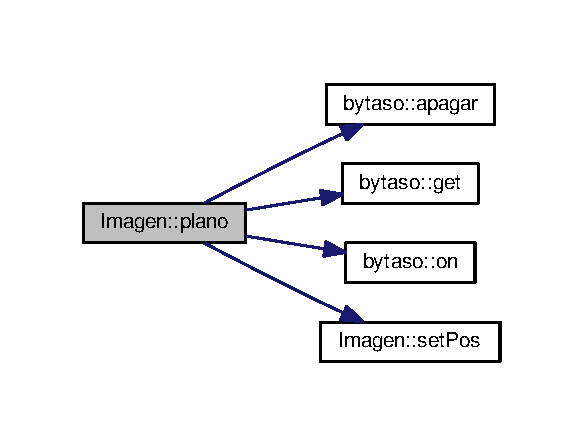
\includegraphics[width=280pt]{class_imagen_a738d3b88a80606af9d78458e5586e04c_cgraph}
\end{center}
\end{figure}




Gráfico de llamadas a esta función\+:
\nopagebreak
\begin{figure}[H]
\begin{center}
\leavevmode
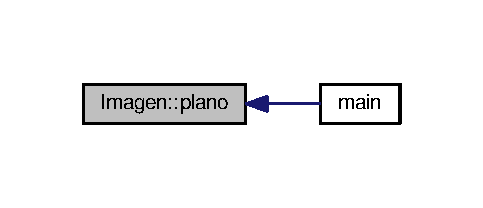
\includegraphics[width=232pt]{class_imagen_a738d3b88a80606af9d78458e5586e04c_icgraph}
\end{center}
\end{figure}


\hypertarget{class_imagen_a722347f0110d794f96c92beda6710158}{}\index{Imagen@{Imagen}!set@{set}}
\index{set@{set}!Imagen@{Imagen}}
\subsubsection[{set(int y, int x, byte v)}]{\setlength{\rightskip}{0pt plus 5cm}void Imagen\+::set (
\begin{DoxyParamCaption}
\item[{int}]{y, }
\item[{int}]{x, }
\item[{{\bf byte}}]{v}
\end{DoxyParamCaption}
)}\label{class_imagen_a722347f0110d794f96c92beda6710158}


Asigna el valor {\itshape v} a la posición ({\itshape x},{\itshape y}) de la imagen. 


\begin{DoxyParams}{Parámetros}
{\em y} & fila de la imagen \\
\hline
{\em x} & columna de la imagen \\
\hline
{\em v} & valor a asignar\\
\hline
\end{DoxyParams}
Asigna el valor {\itshape v} a la posición ({\itshape x},{\itshape y}) de la imagen. Dado que la imagen se guarda como un vector, la posición ({\itshape x},{\itshape y}) corresponde a la posición {\itshape y} $\ast$ {\ttfamily ncolumnas} + {\itshape x} del vector. 

Gráfico de llamadas a esta función\+:
\nopagebreak
\begin{figure}[H]
\begin{center}
\leavevmode
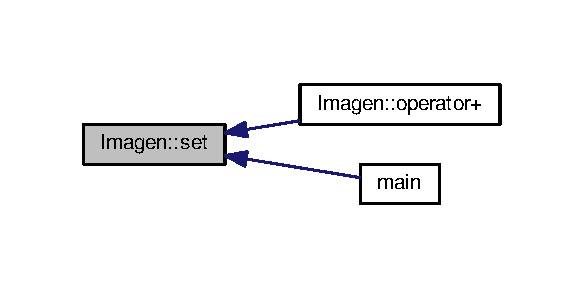
\includegraphics[width=280pt]{class_imagen_a722347f0110d794f96c92beda6710158_icgraph}
\end{center}
\end{figure}


\hypertarget{class_imagen_a9c1bfd9bff6ae8851f3e0c9ac2e90382}{}\index{Imagen@{Imagen}!set\+Pos@{set\+Pos}}
\index{set\+Pos@{set\+Pos}!Imagen@{Imagen}}
\subsubsection[{set\+Pos(int i, byte v)}]{\setlength{\rightskip}{0pt plus 5cm}void Imagen\+::set\+Pos (
\begin{DoxyParamCaption}
\item[{int}]{i, }
\item[{{\bf byte}}]{v}
\end{DoxyParamCaption}
)}\label{class_imagen_a9c1bfd9bff6ae8851f3e0c9ac2e90382}


Asigna el valor {\itshape v} a la posición {\itshape i} de la imagen considerada como vector. 


\begin{DoxyParams}{Parámetros}
{\em i} & posición de la imagen considerada como vector \\
\hline
{\em v} & valor a asignar\\
\hline
\end{DoxyParams}
Asigna el valor {\itshape v} a la posición {\itshape i} de la imagen considerada como vector. La posición {\itshape i} corresponde con la posición {\ttfamily y} $\ast$ {\ttfamily ncolumnas} + {\ttfamily x} de la imagen donde {\ttfamily y} representa la fila y {\ttfamily x} representa la columna. 

Gráfico de llamadas a esta función\+:
\nopagebreak
\begin{figure}[H]
\begin{center}
\leavevmode
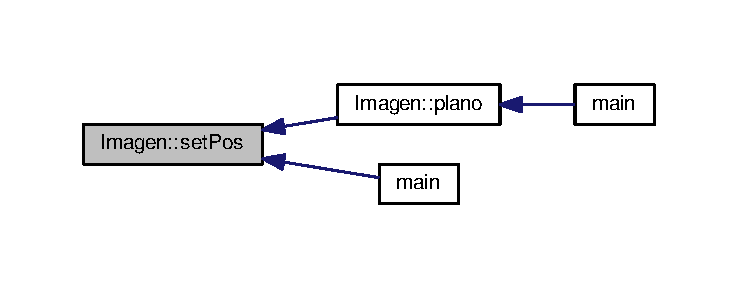
\includegraphics[width=350pt]{class_imagen_a9c1bfd9bff6ae8851f3e0c9ac2e90382_icgraph}
\end{center}
\end{figure}




\subsection{Documentación de los datos miembro}
\hypertarget{class_imagen_a74bf3487e42bb65862e994883fa05b33}{}\index{Imagen@{Imagen}!datos@{datos}}
\index{datos@{datos}!Imagen@{Imagen}}
\subsubsection[{datos}]{\setlength{\rightskip}{0pt plus 5cm}{\bf byte}$\ast$$\ast$ Imagen\+::datos\hspace{0.3cm}{\ttfamily [private]}}\label{class_imagen_a74bf3487e42bb65862e994883fa05b33}


puntero a los punteros de las filas 

\hypertarget{class_imagen_a4b38c0642ab84fe5f945272180ae8306}{}\index{Imagen@{Imagen}!ncolumnas@{ncolumnas}}
\index{ncolumnas@{ncolumnas}!Imagen@{Imagen}}
\subsubsection[{ncolumnas}]{\setlength{\rightskip}{0pt plus 5cm}int Imagen\+::ncolumnas\hspace{0.3cm}{\ttfamily [private]}}\label{class_imagen_a4b38c0642ab84fe5f945272180ae8306}


número de columnsa de la imagen 

\hypertarget{class_imagen_a89599a9692fbe4cb60ee16c0a30a64ef}{}\index{Imagen@{Imagen}!nfilas@{nfilas}}
\index{nfilas@{nfilas}!Imagen@{Imagen}}
\subsubsection[{nfilas}]{\setlength{\rightskip}{0pt plus 5cm}int Imagen\+::nfilas\hspace{0.3cm}{\ttfamily [private]}}\label{class_imagen_a89599a9692fbe4cb60ee16c0a30a64ef}


número de filas de la imagen 



La documentación para esta clase fue generada a partir de los siguientes ficheros\+:\begin{DoxyCompactItemize}
\item 
include/\hyperlink{imagen_8h}{imagen.\+h}\item 
src/\hyperlink{imagen_8cpp}{imagen.\+cpp}\end{DoxyCompactItemize}

\hypertarget{class_lista}{}\section{Referencia de la Clase Lista}
\label{class_lista}\index{Lista@{Lista}}


{\ttfamily \#include $<$lista.\+h$>$}



Diagrama de colaboración para Lista\+:
\nopagebreak
\begin{figure}[H]
\begin{center}
\leavevmode
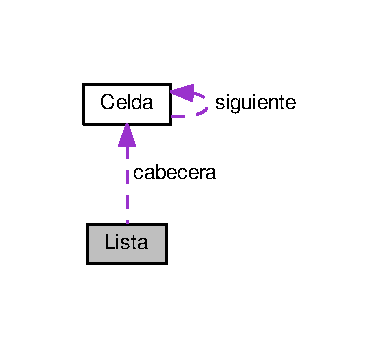
\includegraphics[width=183pt]{class_lista__coll__graph}
\end{center}
\end{figure}
\subsection*{Métodos públicos}
\begin{DoxyCompactItemize}
\item 
\hyperlink{class_lista_a1f668b36909182ef1360b48503529a31}{Lista} ()
\begin{DoxyCompactList}\small\item\em Constructor por defecto. Crea una lista vacía. \end{DoxyCompactList}\item 
\hyperlink{class_lista_a4d7394b2728a00ad8404965b2e15d096}{$\sim$\+Lista} ()
\begin{DoxyCompactList}\small\item\em Destructor. Libera todos los recursos reservados a la lista. \end{DoxyCompactList}\item 
\hyperlink{class_lista_a6a479a165fde4f0b9842d2b26f9fce75}{Lista} (const \hyperlink{class_lista}{Lista} \&)
\begin{DoxyCompactList}\small\item\em Constructor de copia de la clase \hyperlink{class_lista}{Lista}. \end{DoxyCompactList}\item 
\hyperlink{class_lista_adb33dfb3ac2cfef81f52af48afeef0a7}{Lista} (string cadena)
\begin{DoxyCompactList}\small\item\em Construye una lista a partir de un elemento. \end{DoxyCompactList}\item 
void \hyperlink{class_lista_a7b1f5c4b50044823f2746853bfaa5e15}{destruir} ()
\begin{DoxyCompactList}\small\item\em Libera la memoria reservada en la lista de cadenas. \end{DoxyCompactList}\item 
void \hyperlink{class_lista_a2cf31ee7be6ed41e9084efffb807aa5e}{insertar} (string cadena)
\begin{DoxyCompactList}\small\item\em inserta una nueva cadena al final de la lista \end{DoxyCompactList}\item 
string \hyperlink{class_lista_a69c0764aa81aca4543b2a9898d941f51}{get\+Celda} (int i) const 
\begin{DoxyCompactList}\small\item\em devuelve la cadena de la posicion i-\/esima de la lista o una cadena vacia en caso de que el valor de i sea erroneo. \end{DoxyCompactList}\item 
int \hyperlink{class_lista_a445fbaf0a89d99ed9830ae7d0c8dd12f}{longitud} () const 
\begin{DoxyCompactList}\small\item\em devuelve el numero de celdas que contiene la lista \end{DoxyCompactList}\item 
bool \hyperlink{class_lista_aa4be655d8d5ea8e8189e7c577c86b34e}{leer\+Lista} (const char nombrefichero\mbox{[}$\,$\mbox{]})
\begin{DoxyCompactList}\small\item\em Construye una lista de celdas enlazadas a partir de la informacion contenida en un fichero. \end{DoxyCompactList}\item 
\hyperlink{class_lista}{Lista} \& \hyperlink{class_lista_a8e15d78e45d53ef28d3da4f17b245ebc}{operator=} (const \hyperlink{class_lista}{Lista} \&otra)
\begin{DoxyCompactList}\small\item\em Operador de asignación de la clase \hyperlink{class_lista}{Lista}. Si ambos objetos son el mismo se devuelve un puntero a ese sin hacer nada más. \end{DoxyCompactList}\item 
\hyperlink{class_lista}{Lista} \& \hyperlink{class_lista_a01603de447b008cdcbe72828fb7fb806}{operator+} (const string \&s1)
\begin{DoxyCompactList}\small\item\em Operador + de la clase \hyperlink{class_lista}{Lista}. Permite añadir un nuevo string a la lista usando el operador +. \end{DoxyCompactList}\end{DoxyCompactItemize}
\subsection*{Atributos privados}
\begin{DoxyCompactItemize}
\item 
\hyperlink{struct_celda}{Celda} $\ast$ \hyperlink{class_lista_a3a8e4a0637c6c328a00acc4b186f34a2}{cabecera}
\item 
int \hyperlink{class_lista_ad88ae756eb0ea2e6d3046335c5a44db8}{num\+\_\+elementos}
\end{DoxyCompactItemize}


\subsection{Documentación del constructor y destructor}
\hypertarget{class_lista_a1f668b36909182ef1360b48503529a31}{}\index{Lista@{Lista}!Lista@{Lista}}
\index{Lista@{Lista}!Lista@{Lista}}
\subsubsection[{Lista()}]{\setlength{\rightskip}{0pt plus 5cm}Lista\+::\+Lista (
\begin{DoxyParamCaption}
{}
\end{DoxyParamCaption}
)}\label{class_lista_a1f668b36909182ef1360b48503529a31}


Constructor por defecto. Crea una lista vacía. 

\hypertarget{class_lista_a4d7394b2728a00ad8404965b2e15d096}{}\index{Lista@{Lista}!````~Lista@{$\sim$\+Lista}}
\index{````~Lista@{$\sim$\+Lista}!Lista@{Lista}}
\subsubsection[{$\sim$\+Lista()}]{\setlength{\rightskip}{0pt plus 5cm}Lista\+::$\sim$\+Lista (
\begin{DoxyParamCaption}
{}
\end{DoxyParamCaption}
)}\label{class_lista_a4d7394b2728a00ad8404965b2e15d096}


Destructor. Libera todos los recursos reservados a la lista. 

\hypertarget{class_lista_a6a479a165fde4f0b9842d2b26f9fce75}{}\index{Lista@{Lista}!Lista@{Lista}}
\index{Lista@{Lista}!Lista@{Lista}}
\subsubsection[{Lista(const Lista \&)}]{\setlength{\rightskip}{0pt plus 5cm}Lista\+::\+Lista (
\begin{DoxyParamCaption}
\item[{const {\bf Lista} \&}]{otra}
\end{DoxyParamCaption}
)}\label{class_lista_a6a479a165fde4f0b9842d2b26f9fce75}


Constructor de copia de la clase \hyperlink{class_lista}{Lista}. 

\hypertarget{class_lista_adb33dfb3ac2cfef81f52af48afeef0a7}{}\index{Lista@{Lista}!Lista@{Lista}}
\index{Lista@{Lista}!Lista@{Lista}}
\subsubsection[{Lista(string cadena)}]{\setlength{\rightskip}{0pt plus 5cm}Lista\+::\+Lista (
\begin{DoxyParamCaption}
\item[{string}]{cadena}
\end{DoxyParamCaption}
)}\label{class_lista_adb33dfb3ac2cfef81f52af48afeef0a7}


Construye una lista a partir de un elemento. 


\begin{DoxyParams}{Parámetros}
{\em cadena} & el elemento a insertar en la lista\\
\hline
\end{DoxyParams}
Construye una lista de tamaño 1 e inserta la cadena {\itshape cadena} 

\subsection{Documentación de las funciones miembro}
\hypertarget{class_lista_a7b1f5c4b50044823f2746853bfaa5e15}{}\index{Lista@{Lista}!destruir@{destruir}}
\index{destruir@{destruir}!Lista@{Lista}}
\subsubsection[{destruir()}]{\setlength{\rightskip}{0pt plus 5cm}void Lista\+::destruir (
\begin{DoxyParamCaption}
{}
\end{DoxyParamCaption}
)}\label{class_lista_a7b1f5c4b50044823f2746853bfaa5e15}


Libera la memoria reservada en la lista de cadenas. 

Libera la memoria reservada en el vetor de imagen y actualiza el numero de elementos de la misma a 0. \hypertarget{class_lista_a69c0764aa81aca4543b2a9898d941f51}{}\index{Lista@{Lista}!get\+Celda@{get\+Celda}}
\index{get\+Celda@{get\+Celda}!Lista@{Lista}}
\subsubsection[{get\+Celda(int i) const }]{\setlength{\rightskip}{0pt plus 5cm}string Lista\+::get\+Celda (
\begin{DoxyParamCaption}
\item[{int}]{i}
\end{DoxyParamCaption}
) const}\label{class_lista_a69c0764aa81aca4543b2a9898d941f51}


devuelve la cadena de la posicion i-\/esima de la lista o una cadena vacia en caso de que el valor de i sea erroneo. 


\begin{DoxyParams}{Parámetros}
{\em i} & indice del elemento dentro de la lista \\
\hline
\end{DoxyParams}
\begin{DoxyPrecond}{Precondición}
i debe ser menor que el tamaño total de la lista. 
\end{DoxyPrecond}
\begin{DoxyReturn}{Devuelve}
la cadena que se encuentra en la celda con indice {\itshape i} siempre que este valor se encuentre en los margenes de la lista, o una cadena vacia en caso contrario 
\end{DoxyReturn}


Gráfico de llamadas a esta función\+:
\nopagebreak
\begin{figure}[H]
\begin{center}
\leavevmode
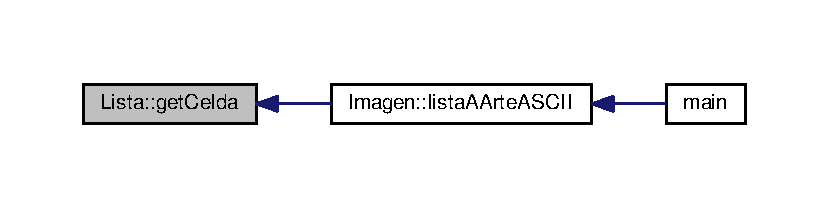
\includegraphics[width=350pt]{class_lista_a69c0764aa81aca4543b2a9898d941f51_icgraph}
\end{center}
\end{figure}


\hypertarget{class_lista_a2cf31ee7be6ed41e9084efffb807aa5e}{}\index{Lista@{Lista}!insertar@{insertar}}
\index{insertar@{insertar}!Lista@{Lista}}
\subsubsection[{insertar(string cadena)}]{\setlength{\rightskip}{0pt plus 5cm}void Lista\+::insertar (
\begin{DoxyParamCaption}
\item[{string}]{cadena}
\end{DoxyParamCaption}
)}\label{class_lista_a2cf31ee7be6ed41e9084efffb807aa5e}


inserta una nueva cadena al final de la lista 


\begin{DoxyParams}{Parámetros}
{\em cad} & elemento a insertar en la lista\\
\hline
\end{DoxyParams}
Añade un nuevo elemento ( {\itshape cadena} ) a la lista 

Gráfico de llamadas a esta función\+:
\nopagebreak
\begin{figure}[H]
\begin{center}
\leavevmode
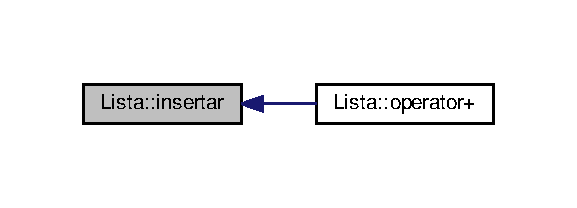
\includegraphics[width=277pt]{class_lista_a2cf31ee7be6ed41e9084efffb807aa5e_icgraph}
\end{center}
\end{figure}


\hypertarget{class_lista_aa4be655d8d5ea8e8189e7c577c86b34e}{}\index{Lista@{Lista}!leer\+Lista@{leer\+Lista}}
\index{leer\+Lista@{leer\+Lista}!Lista@{Lista}}
\subsubsection[{leer\+Lista(const char nombrefichero[])}]{\setlength{\rightskip}{0pt plus 5cm}bool Lista\+::leer\+Lista (
\begin{DoxyParamCaption}
\item[{const char}]{nombrefichero\mbox{[}$\,$\mbox{]}}
\end{DoxyParamCaption}
)}\label{class_lista_aa4be655d8d5ea8e8189e7c577c86b34e}


Construye una lista de celdas enlazadas a partir de la informacion contenida en un fichero. 


\begin{DoxyParams}{Parámetros}
{\em nombre\+Fichero} & ruta del fichero de texto con el contenido de las cadenas a insertar en la lista \\
\hline
\end{DoxyParams}

\begin{DoxyRetVals}{Valores devueltos}
{\em true} & si ha tenido éxito en la lectura y el formato es el correcto \\
\hline
{\em false} & si se ha producido algún error en la lectura\\
\hline
\end{DoxyRetVals}
Lee desde disco los elementos almacenados en {\itshape nombre\+Fichero} y los guarda en la lista. La función debe asegurarse de que la estructura sigue un patron determinado, y se ha de crear la lista con el numero de elementos que contenga.


\begin{DoxyParams}{Parámetros}
{\em nombre\+Fichero} & ruta del fichero de texto con el contenido de las datoss a insertar en la lista \\
\hline
\end{DoxyParams}

\begin{DoxyRetVals}{Valores devueltos}
{\em true} & si ha tenido éxito en la lectura y el formato es el correcto \\
\hline
{\em false} & si se ha producido algún error en la lectura\\
\hline
\end{DoxyRetVals}
Lee desde disco los elementos almacenados en {\itshape nombre\+Fichero} y los guarda en la lista. La función debe asegurarse de que la estructura sigue un patron determinado, y se ha de crear la lista con el numero de elementos que contenga. 

Gráfico de llamadas a esta función\+:
\nopagebreak
\begin{figure}[H]
\begin{center}
\leavevmode
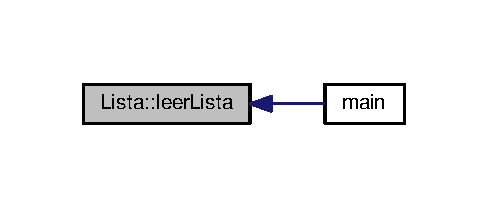
\includegraphics[width=234pt]{class_lista_aa4be655d8d5ea8e8189e7c577c86b34e_icgraph}
\end{center}
\end{figure}


\hypertarget{class_lista_a445fbaf0a89d99ed9830ae7d0c8dd12f}{}\index{Lista@{Lista}!longitud@{longitud}}
\index{longitud@{longitud}!Lista@{Lista}}
\subsubsection[{longitud() const }]{\setlength{\rightskip}{0pt plus 5cm}int Lista\+::longitud (
\begin{DoxyParamCaption}
{}
\end{DoxyParamCaption}
) const}\label{class_lista_a445fbaf0a89d99ed9830ae7d0c8dd12f}


devuelve el numero de celdas que contiene la lista 

\begin{DoxyReturn}{Devuelve}
el tamaño de la lista 
\end{DoxyReturn}


Gráfico de llamadas a esta función\+:
\nopagebreak
\begin{figure}[H]
\begin{center}
\leavevmode
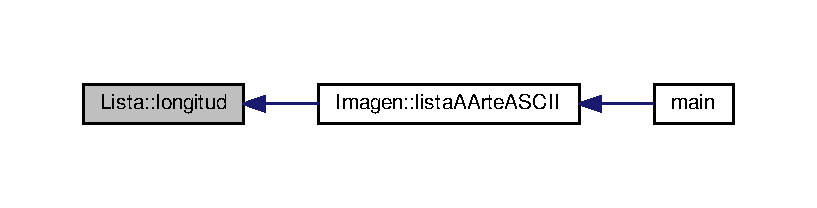
\includegraphics[width=350pt]{class_lista_a445fbaf0a89d99ed9830ae7d0c8dd12f_icgraph}
\end{center}
\end{figure}


\hypertarget{class_lista_a01603de447b008cdcbe72828fb7fb806}{}\index{Lista@{Lista}!operator+@{operator+}}
\index{operator+@{operator+}!Lista@{Lista}}
\subsubsection[{operator+(const string \&s1)}]{\setlength{\rightskip}{0pt plus 5cm}{\bf Lista} \& Lista\+::operator+ (
\begin{DoxyParamCaption}
\item[{const string \&}]{s1}
\end{DoxyParamCaption}
)}\label{class_lista_a01603de447b008cdcbe72828fb7fb806}


Operador + de la clase \hyperlink{class_lista}{Lista}. Permite añadir un nuevo string a la lista usando el operador +. 


\begin{DoxyParams}{Parámetros}
{\em String} & a añadir \\
\hline
\end{DoxyParams}
\begin{DoxyReturn}{Devuelve}
Puntero a la lista ya modificada. 
\end{DoxyReturn}


Gráfico de llamadas para esta función\+:
\nopagebreak
\begin{figure}[H]
\begin{center}
\leavevmode
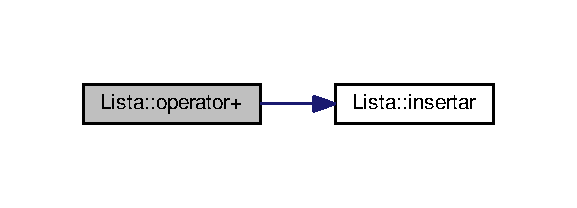
\includegraphics[width=277pt]{class_lista_a01603de447b008cdcbe72828fb7fb806_cgraph}
\end{center}
\end{figure}


\hypertarget{class_lista_a8e15d78e45d53ef28d3da4f17b245ebc}{}\index{Lista@{Lista}!operator=@{operator=}}
\index{operator=@{operator=}!Lista@{Lista}}
\subsubsection[{operator=(const Lista \&otra)}]{\setlength{\rightskip}{0pt plus 5cm}{\bf Lista} \& Lista\+::operator= (
\begin{DoxyParamCaption}
\item[{const {\bf Lista} \&}]{otra}
\end{DoxyParamCaption}
)}\label{class_lista_a8e15d78e45d53ef28d3da4f17b245ebc}


Operador de asignación de la clase \hyperlink{class_lista}{Lista}. Si ambos objetos son el mismo se devuelve un puntero a ese sin hacer nada más. 


\begin{DoxyParams}{Parámetros}
{\em \hyperlink{class_lista}{Lista}} & a copiar \\
\hline
\end{DoxyParams}
\begin{DoxyReturn}{Devuelve}
puntero a la lista recién asignada. 
\end{DoxyReturn}


\subsection{Documentación de los datos miembro}
\hypertarget{class_lista_a3a8e4a0637c6c328a00acc4b186f34a2}{}\index{Lista@{Lista}!cabecera@{cabecera}}
\index{cabecera@{cabecera}!Lista@{Lista}}
\subsubsection[{cabecera}]{\setlength{\rightskip}{0pt plus 5cm}{\bf Celda}$\ast$ Lista\+::cabecera\hspace{0.3cm}{\ttfamily [private]}}\label{class_lista_a3a8e4a0637c6c328a00acc4b186f34a2}
\hypertarget{class_lista_ad88ae756eb0ea2e6d3046335c5a44db8}{}\index{Lista@{Lista}!num\+\_\+elementos@{num\+\_\+elementos}}
\index{num\+\_\+elementos@{num\+\_\+elementos}!Lista@{Lista}}
\subsubsection[{num\+\_\+elementos}]{\setlength{\rightskip}{0pt plus 5cm}int Lista\+::num\+\_\+elementos\hspace{0.3cm}{\ttfamily [private]}}\label{class_lista_ad88ae756eb0ea2e6d3046335c5a44db8}


La documentación para esta clase fue generada a partir de los siguientes ficheros\+:\begin{DoxyCompactItemize}
\item 
include/\hyperlink{lista_8h}{lista.\+h}\item 
src/\hyperlink{lista_8cpp}{lista.\+cpp}\end{DoxyCompactItemize}

\chapter{Documentación de archivos}
\hypertarget{byte_8h}{}\section{Referencia del Archivo include/byte.h}
\label{byte_8h}\index{include/byte.\+h@{include/byte.\+h}}


Funciones de manejo de bytes.  


{\ttfamily \#include $<$iostream$>$}\\*
{\ttfamily \#include $<$string$>$}\\*
Dependencia gráfica adjunta para byte.\+h\+:
\nopagebreak
\begin{figure}[H]
\begin{center}
\leavevmode
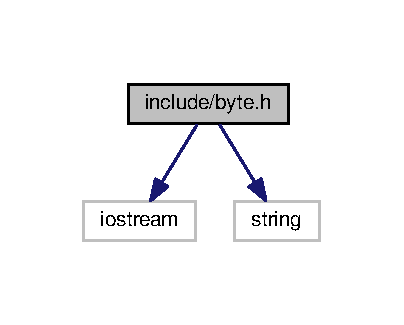
\includegraphics[width=194pt]{byte_8h__incl}
\end{center}
\end{figure}
Gráfico de los archivos que directa o indirectamente incluyen a este archivo\+:
\nopagebreak
\begin{figure}[H]
\begin{center}
\leavevmode
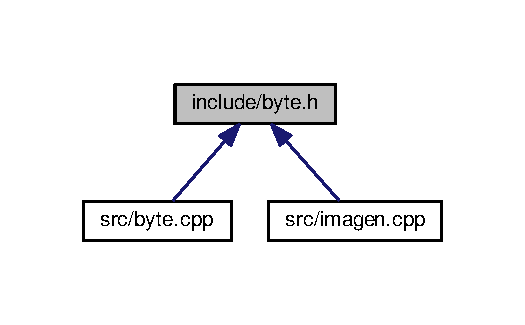
\includegraphics[width=252pt]{byte_8h__dep__incl}
\end{center}
\end{figure}
\subsection*{Namespaces}
\begin{DoxyCompactItemize}
\item 
 \hyperlink{namespacebytaso}{bytaso}
\end{DoxyCompactItemize}
\subsection*{\textquotesingle{}typedefs\textquotesingle{}}
\begin{DoxyCompactItemize}
\item 
typedef unsigned char \hyperlink{namespacebytaso_a02813d6c4d42ce94319af7feabc46476}{bytaso\+::byte}
\begin{DoxyCompactList}\small\item\em Un {\ttfamily byte} contiene el estado de 8 bits. \end{DoxyCompactList}\end{DoxyCompactItemize}
\subsection*{Funciones}
\begin{DoxyCompactItemize}
\item 
void \hyperlink{namespacebytaso_ae98a18093e63134e5f1ddec44973c6ec}{bytaso\+::on} (\hyperlink{imagen_8h_a0c8186d9b9b7880309c27230bbb5e69d}{byte} \&b, int pos)
\begin{DoxyCompactList}\small\item\em enciende el bit {\ttfamily pos} del {\ttfamily byte} {\ttfamily b} \end{DoxyCompactList}\item 
void \hyperlink{namespacebytaso_a477a14f602dcc9264dbb6f874d170834}{bytaso\+::off} (\hyperlink{imagen_8h_a0c8186d9b9b7880309c27230bbb5e69d}{byte} \&b, int pos)
\begin{DoxyCompactList}\small\item\em apaga el bit {\ttfamily pos} del {\ttfamily byte} {\ttfamily b} \end{DoxyCompactList}\item 
bool \hyperlink{namespacebytaso_ad231ba96547f99130292527f5d65694b}{bytaso\+::get} (\hyperlink{imagen_8h_a0c8186d9b9b7880309c27230bbb5e69d}{byte} b, int pos)
\begin{DoxyCompactList}\small\item\em devuelve el estado del bit (encendido = true, apagado = false) en la posici�n {\ttfamily pos} \end{DoxyCompactList}\item 
string \hyperlink{namespacebytaso_a01303edb3c075bbf9f10324914352a50}{bytaso\+::byte\+To\+String} (\hyperlink{imagen_8h_a0c8186d9b9b7880309c27230bbb5e69d}{byte} b)
\begin{DoxyCompactList}\small\item\em Muestra por la salida est�ndar una secuencia de 0s y 1s correspondiente al estado de cada bit. \end{DoxyCompactList}\item 
void \hyperlink{namespacebytaso_a5e016205a37415abe06efd845593bc2a}{bytaso\+::encender} (\hyperlink{imagen_8h_a0c8186d9b9b7880309c27230bbb5e69d}{byte} \&b)
\begin{DoxyCompactList}\small\item\em enciende todos los bits \end{DoxyCompactList}\item 
void \hyperlink{namespacebytaso_a29bc6fb2d3ca8a24ee9a8fc044aed54a}{bytaso\+::apagar} (\hyperlink{imagen_8h_a0c8186d9b9b7880309c27230bbb5e69d}{byte} \&b)
\begin{DoxyCompactList}\small\item\em apaga todos los bits \end{DoxyCompactList}\item 
void \hyperlink{namespacebytaso_ae93ec524c1a740b4144a2ec249d07446}{bytaso\+::asignar} (\hyperlink{imagen_8h_a0c8186d9b9b7880309c27230bbb5e69d}{byte} \&b, const bool v\mbox{[}$\,$\mbox{]})
\begin{DoxyCompactList}\small\item\em enciende los bits seg�n la configuraci�n de {\ttfamily v} \end{DoxyCompactList}\item 
void \hyperlink{namespacebytaso_aca892e499e255f8b8a967b67cd164a75}{bytaso\+::volcar} (\hyperlink{imagen_8h_a0c8186d9b9b7880309c27230bbb5e69d}{byte} b, bool v\mbox{[}$\,$\mbox{]})
\begin{DoxyCompactList}\small\item\em recupera la configuraci�n de todos los bit \end{DoxyCompactList}\item 
void \hyperlink{namespacebytaso_a76ad23326440e16a7b419ee7a14ee287}{bytaso\+::encendidos} (\hyperlink{imagen_8h_a0c8186d9b9b7880309c27230bbb5e69d}{byte} b, int posic\mbox{[}$\,$\mbox{]}, int \&cuantos)
\begin{DoxyCompactList}\small\item\em devuelve las posiciones de los bits encendidos \end{DoxyCompactList}\end{DoxyCompactItemize}


\subsection{Descripción detallada}
Funciones de manejo de bytes. 

\begin{DoxyAuthor}{Autor}
Ra�l Mart�n Pineda \& Jose Manuel Linares Rojas 
\end{DoxyAuthor}
\begin{DoxyDate}{Fecha}
18 de marzo de 2016, 10\+:15 
\end{DoxyDate}

\hypertarget{imagen_8h}{}\section{Referencia del Archivo include/imagen.h}
\label{imagen_8h}\index{include/imagen.\+h@{include/imagen.\+h}}


Clase imagen blanco y negro.  


{\ttfamily \#include \char`\"{}lista.\+h\char`\"{}}\\*
Dependencia gráfica adjunta para imagen.\+h\+:
\nopagebreak
\begin{figure}[H]
\begin{center}
\leavevmode
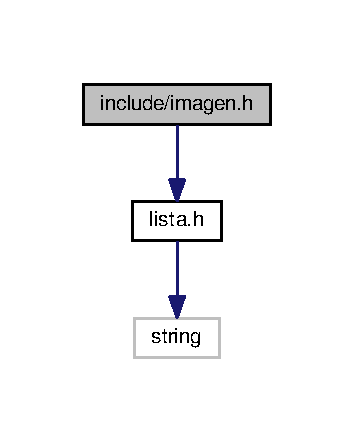
\includegraphics[width=170pt]{imagen_8h__incl}
\end{center}
\end{figure}
Gráfico de los archivos que directa o indirectamente incluyen a este archivo\+:
\nopagebreak
\begin{figure}[H]
\begin{center}
\leavevmode
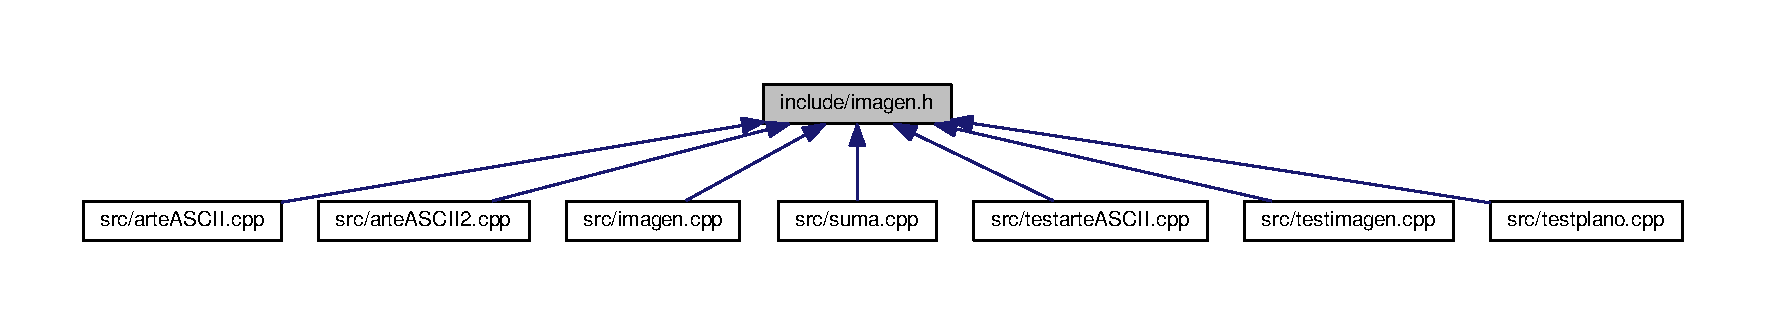
\includegraphics[width=350pt]{imagen_8h__dep__incl}
\end{center}
\end{figure}
\subsection*{Clases}
\begin{DoxyCompactItemize}
\item 
class \hyperlink{class_imagen}{Imagen}
\begin{DoxyCompactList}\small\item\em Una imagen en blanco y negro. Cada píxel es un byte. \end{DoxyCompactList}\end{DoxyCompactItemize}
\subsection*{\textquotesingle{}typedefs\textquotesingle{}}
\begin{DoxyCompactItemize}
\item 
typedef unsigned char \hyperlink{imagen_8h_a0c8186d9b9b7880309c27230bbb5e69d}{byte}
\begin{DoxyCompactList}\small\item\em byte = 8bits almacenado en un unsigned char \end{DoxyCompactList}\end{DoxyCompactItemize}


\subsection{Descripción detallada}
Clase imagen blanco y negro. 



\subsection{Documentación de los \textquotesingle{}typedefs\textquotesingle{}}
\hypertarget{imagen_8h_a0c8186d9b9b7880309c27230bbb5e69d}{}\index{imagen.\+h@{imagen.\+h}!byte@{byte}}
\index{byte@{byte}!imagen.\+h@{imagen.\+h}}
\subsubsection[{byte}]{\setlength{\rightskip}{0pt plus 5cm}typedef unsigned char {\bf byte}}\label{imagen_8h_a0c8186d9b9b7880309c27230bbb5e69d}


byte = 8bits almacenado en un unsigned char 


\hypertarget{lista_8h}{}\section{Referencia del Archivo include/lista.h}
\label{lista_8h}\index{include/lista.\+h@{include/lista.\+h}}


Clase para la estructura de datos de lista de strings.  


{\ttfamily \#include $<$string$>$}\\*
Dependencia gráfica adjunta para lista.\+h\+:
\nopagebreak
\begin{figure}[H]
\begin{center}
\leavevmode
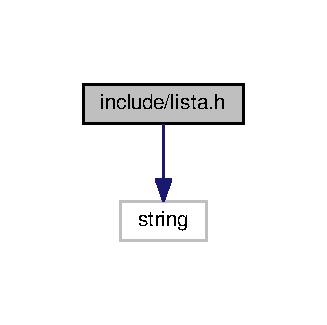
\includegraphics[width=157pt]{lista_8h__incl}
\end{center}
\end{figure}
Gráfico de los archivos que directa o indirectamente incluyen a este archivo\+:
\nopagebreak
\begin{figure}[H]
\begin{center}
\leavevmode
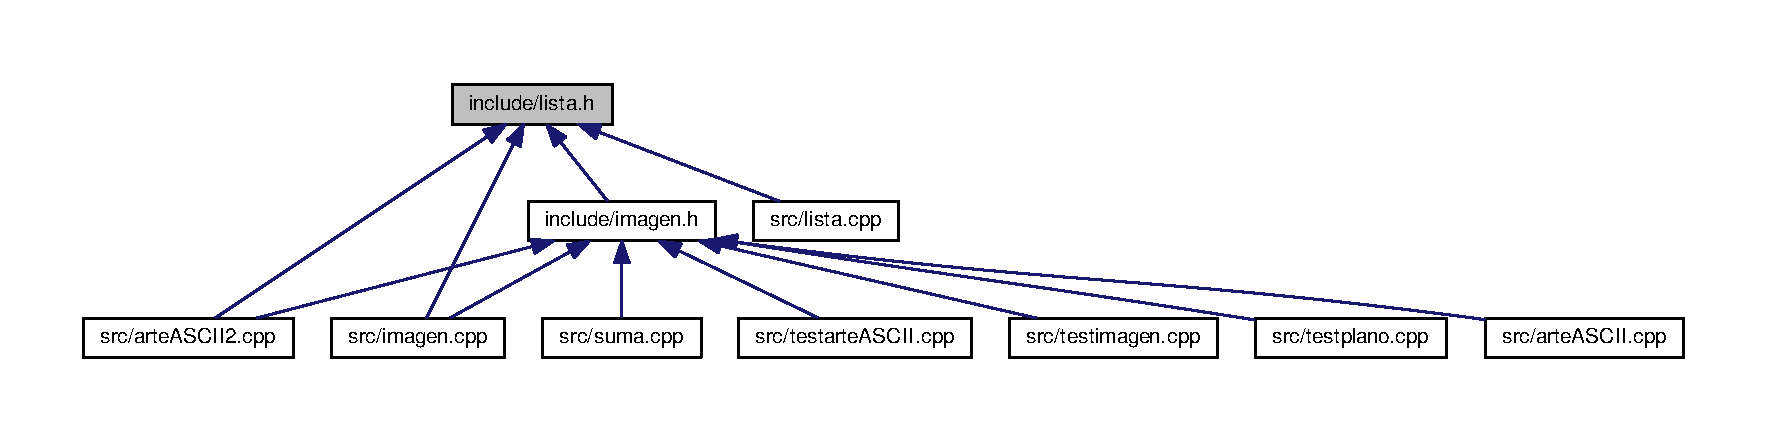
\includegraphics[width=350pt]{lista_8h__dep__incl}
\end{center}
\end{figure}
\subsection*{Clases}
\begin{DoxyCompactItemize}
\item 
struct \hyperlink{struct_celda}{Celda}
\item 
class \hyperlink{class_lista}{Lista}
\end{DoxyCompactItemize}


\subsection{Descripción detallada}
Clase para la estructura de datos de lista de strings. 

Permite el manejo de cadenas (strings) en una lista enlazada 
\hypertarget{pgm_8h}{}\section{Referencia del Archivo include/pgm.h}
\label{pgm_8h}\index{include/pgm.\+h@{include/pgm.\+h}}


Fichero cabecera para la E/\+S de imágenes P\+G\+M.  


Gráfico de los archivos que directa o indirectamente incluyen a este archivo\+:
\nopagebreak
\begin{figure}[H]
\begin{center}
\leavevmode
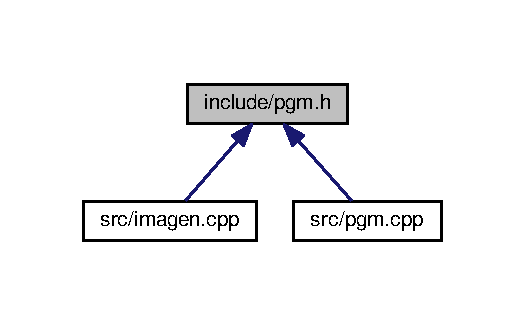
\includegraphics[width=252pt]{pgm_8h__dep__incl}
\end{center}
\end{figure}
\subsection*{Enumeraciones}
\begin{DoxyCompactItemize}
\item 
enum \hyperlink{pgm_8h_a8914f6544a484741b05c092d9e7522ed}{Tipo\+Imagen} \{ \hyperlink{pgm_8h_a8914f6544a484741b05c092d9e7522eda23c8d70e6eadf2d0d0ee1fd3bb293384}{I\+M\+G\+\_\+\+D\+E\+S\+C\+O\+N\+O\+C\+I\+D\+O}, 
\hyperlink{pgm_8h_a8914f6544a484741b05c092d9e7522eda724f6134dce25e3d82af96f9061dd9de}{I\+M\+G\+\_\+\+P\+G\+M\+\_\+\+B\+I\+N\+A\+R\+I\+O}, 
\hyperlink{pgm_8h_a8914f6544a484741b05c092d9e7522eda2535c521166366e04b5091ef8acfcbde}{I\+M\+G\+\_\+\+P\+G\+M\+\_\+\+T\+E\+X\+T\+O}
 \}\begin{DoxyCompactList}\small\item\em Tipo de imagen. \end{DoxyCompactList}
\end{DoxyCompactItemize}
\subsection*{Funciones}
\begin{DoxyCompactItemize}
\item 
\hyperlink{pgm_8h_a8914f6544a484741b05c092d9e7522ed}{Tipo\+Imagen} \hyperlink{pgm_8h_a85c7f15bdcdee461eba76965aaccb910}{info\+P\+G\+M} (const char nombre\mbox{[}$\,$\mbox{]}, int \&filas, int \&columnas)
\begin{DoxyCompactList}\small\item\em Consulta el tipo de imagen del archivo y sus dimensiones. \end{DoxyCompactList}\item 
bool \hyperlink{pgm_8h_a3d11aef73fef65e3ba31446f8fc20595}{leer\+P\+G\+M\+Binario} (const char nombre\mbox{[}$\,$\mbox{]}, unsigned char datos\mbox{[}$\,$\mbox{]}, int \&filas, int \&columnas)
\begin{DoxyCompactList}\small\item\em Lee una imagen de tipo P\+G\+M binario. \end{DoxyCompactList}\item 
bool \hyperlink{pgm_8h_a381cd69ce2e9de0b0e3b12131a397121}{escribir\+P\+G\+M\+Binario} (const char nombre\mbox{[}$\,$\mbox{]}, const unsigned char datos\mbox{[}$\,$\mbox{]}, int filas, int columnas)
\begin{DoxyCompactList}\small\item\em Escribe una imagen de tipo P\+G\+M binario. \end{DoxyCompactList}\item 
bool \hyperlink{pgm_8h_ad0376e7bb607f570d680118ef291ee3d}{leer\+P\+G\+M\+Texto} (const char nombre\mbox{[}$\,$\mbox{]}, unsigned char datos\mbox{[}$\,$\mbox{]}, int \&filas, int \&columnas)
\item 
bool \hyperlink{pgm_8h_a0ecaed351740580902d90a4c496a0e3b}{escribir\+P\+G\+M\+Texto} (const char nombre\mbox{[}$\,$\mbox{]}, const unsigned char datos\mbox{[}$\,$\mbox{]}, int filas, int columnas)
\end{DoxyCompactItemize}


\subsection{Descripción detallada}
Fichero cabecera para la E/\+S de imágenes P\+G\+M. 

Permite la E/\+S de archivos de tipos P\+G\+M 

\subsection{Documentación de las enumeraciones}
\hypertarget{pgm_8h_a8914f6544a484741b05c092d9e7522ed}{}\index{pgm.\+h@{pgm.\+h}!Tipo\+Imagen@{Tipo\+Imagen}}
\index{Tipo\+Imagen@{Tipo\+Imagen}!pgm.\+h@{pgm.\+h}}
\subsubsection[{Tipo\+Imagen}]{\setlength{\rightskip}{0pt plus 5cm}enum {\bf Tipo\+Imagen}}\label{pgm_8h_a8914f6544a484741b05c092d9e7522ed}


Tipo de imagen. 

Declara una serie de constantes para representar los distintos tipos de imágenes que se pueden manejar.

\begin{DoxySeeAlso}{Ver también}
Leer\+Tipo\+Imagen 
\end{DoxySeeAlso}
\begin{Desc}
\item[Valores de enumeraciones]\par
\begin{description}
\index{I\+M\+G\+\_\+\+D\+E\+S\+C\+O\+N\+O\+C\+I\+D\+O@{I\+M\+G\+\_\+\+D\+E\+S\+C\+O\+N\+O\+C\+I\+D\+O}!pgm.\+h@{pgm.\+h}}\index{pgm.\+h@{pgm.\+h}!I\+M\+G\+\_\+\+D\+E\+S\+C\+O\+N\+O\+C\+I\+D\+O@{I\+M\+G\+\_\+\+D\+E\+S\+C\+O\+N\+O\+C\+I\+D\+O}}\item[{\em 
\hypertarget{pgm_8h_a8914f6544a484741b05c092d9e7522eda23c8d70e6eadf2d0d0ee1fd3bb293384}{}I\+M\+G\+\_\+\+D\+E\+S\+C\+O\+N\+O\+C\+I\+D\+O\label{pgm_8h_a8914f6544a484741b05c092d9e7522eda23c8d70e6eadf2d0d0ee1fd3bb293384}
}]Tipo de imagen desconocido. \index{I\+M\+G\+\_\+\+P\+G\+M\+\_\+\+B\+I\+N\+A\+R\+I\+O@{I\+M\+G\+\_\+\+P\+G\+M\+\_\+\+B\+I\+N\+A\+R\+I\+O}!pgm.\+h@{pgm.\+h}}\index{pgm.\+h@{pgm.\+h}!I\+M\+G\+\_\+\+P\+G\+M\+\_\+\+B\+I\+N\+A\+R\+I\+O@{I\+M\+G\+\_\+\+P\+G\+M\+\_\+\+B\+I\+N\+A\+R\+I\+O}}\item[{\em 
\hypertarget{pgm_8h_a8914f6544a484741b05c092d9e7522eda724f6134dce25e3d82af96f9061dd9de}{}I\+M\+G\+\_\+\+P\+G\+M\+\_\+\+B\+I\+N\+A\+R\+I\+O\label{pgm_8h_a8914f6544a484741b05c092d9e7522eda724f6134dce25e3d82af96f9061dd9de}
}]\hyperlink{class_imagen}{Imagen} tipo P\+G\+M Binario. \index{I\+M\+G\+\_\+\+P\+G\+M\+\_\+\+T\+E\+X\+T\+O@{I\+M\+G\+\_\+\+P\+G\+M\+\_\+\+T\+E\+X\+T\+O}!pgm.\+h@{pgm.\+h}}\index{pgm.\+h@{pgm.\+h}!I\+M\+G\+\_\+\+P\+G\+M\+\_\+\+T\+E\+X\+T\+O@{I\+M\+G\+\_\+\+P\+G\+M\+\_\+\+T\+E\+X\+T\+O}}\item[{\em 
\hypertarget{pgm_8h_a8914f6544a484741b05c092d9e7522eda2535c521166366e04b5091ef8acfcbde}{}I\+M\+G\+\_\+\+P\+G\+M\+\_\+\+T\+E\+X\+T\+O\label{pgm_8h_a8914f6544a484741b05c092d9e7522eda2535c521166366e04b5091ef8acfcbde}
}]\hyperlink{class_imagen}{Imagen} tipo P\+G\+M Texto. \end{description}
\end{Desc}


\subsection{Documentación de las funciones}
\hypertarget{pgm_8h_a381cd69ce2e9de0b0e3b12131a397121}{}\index{pgm.\+h@{pgm.\+h}!escribir\+P\+G\+M\+Binario@{escribir\+P\+G\+M\+Binario}}
\index{escribir\+P\+G\+M\+Binario@{escribir\+P\+G\+M\+Binario}!pgm.\+h@{pgm.\+h}}
\subsubsection[{escribir\+P\+G\+M\+Binario(const char nombre[], const unsigned char datos[], int filas, int columnas)}]{\setlength{\rightskip}{0pt plus 5cm}bool escribir\+P\+G\+M\+Binario (
\begin{DoxyParamCaption}
\item[{const char}]{nombre\mbox{[}$\,$\mbox{]}, }
\item[{const unsigned char}]{datos\mbox{[}$\,$\mbox{]}, }
\item[{int}]{filas, }
\item[{int}]{columnas}
\end{DoxyParamCaption}
)}\label{pgm_8h_a381cd69ce2e9de0b0e3b12131a397121}


Escribe una imagen de tipo P\+G\+M binario. 


\begin{DoxyParams}{Parámetros}
{\em nombre} & nombre del archivo a escribir \\
\hline
{\em datos} & vector con {\itshape filas} x {\itshape columnas} bytes que corresponden a los valores de los píxeles de la imagen de grises. \\
\hline
{\em filas} & número de filas de la imagen \\
\hline
{\em columnas} & número de columnas de la imagen \\
\hline
\end{DoxyParams}

\begin{DoxyRetVals}{Valores devueltos}
{\em true} & si ha tenido éxito en la escritura. \\
\hline
{\em false} & si se ha producido algún error en la escritura. \\
\hline
\end{DoxyRetVals}


Gráfico de llamadas a esta función\+:
\nopagebreak
\begin{figure}[H]
\begin{center}
\leavevmode
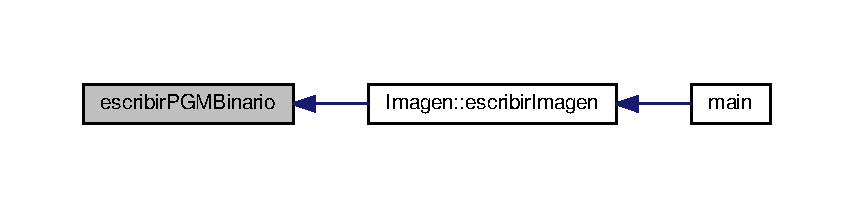
\includegraphics[width=350pt]{pgm_8h_a381cd69ce2e9de0b0e3b12131a397121_icgraph}
\end{center}
\end{figure}


\hypertarget{pgm_8h_a0ecaed351740580902d90a4c496a0e3b}{}\index{pgm.\+h@{pgm.\+h}!escribir\+P\+G\+M\+Texto@{escribir\+P\+G\+M\+Texto}}
\index{escribir\+P\+G\+M\+Texto@{escribir\+P\+G\+M\+Texto}!pgm.\+h@{pgm.\+h}}
\subsubsection[{escribir\+P\+G\+M\+Texto(const char nombre[], const unsigned char datos[], int filas, int columnas)}]{\setlength{\rightskip}{0pt plus 5cm}bool escribir\+P\+G\+M\+Texto (
\begin{DoxyParamCaption}
\item[{const char}]{nombre\mbox{[}$\,$\mbox{]}, }
\item[{const unsigned char}]{datos\mbox{[}$\,$\mbox{]}, }
\item[{int}]{filas, }
\item[{int}]{columnas}
\end{DoxyParamCaption}
)}\label{pgm_8h_a0ecaed351740580902d90a4c496a0e3b}


Gráfico de llamadas a esta función\+:
\nopagebreak
\begin{figure}[H]
\begin{center}
\leavevmode
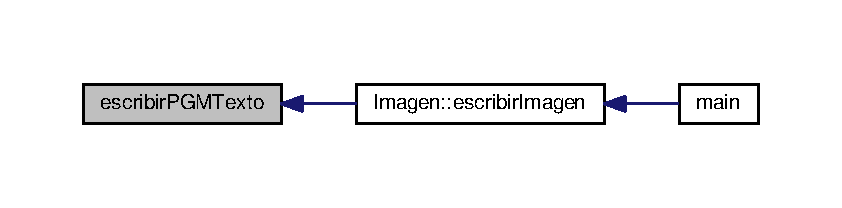
\includegraphics[width=350pt]{pgm_8h_a0ecaed351740580902d90a4c496a0e3b_icgraph}
\end{center}
\end{figure}


\hypertarget{pgm_8h_a85c7f15bdcdee461eba76965aaccb910}{}\index{pgm.\+h@{pgm.\+h}!info\+P\+G\+M@{info\+P\+G\+M}}
\index{info\+P\+G\+M@{info\+P\+G\+M}!pgm.\+h@{pgm.\+h}}
\subsubsection[{info\+P\+G\+M(const char nombre[], int \&filas, int \&columnas)}]{\setlength{\rightskip}{0pt plus 5cm}{\bf Tipo\+Imagen} info\+P\+G\+M (
\begin{DoxyParamCaption}
\item[{const char}]{nombre\mbox{[}$\,$\mbox{]}, }
\item[{int \&}]{filas, }
\item[{int \&}]{columnas}
\end{DoxyParamCaption}
)}\label{pgm_8h_a85c7f15bdcdee461eba76965aaccb910}


Consulta el tipo de imagen del archivo y sus dimensiones. 


\begin{DoxyParams}{Parámetros}
{\em nombre} & indica el nombre del archivo de disco a consultar \\
\hline
{\em filas} & Parámetro de salida con las filas de la imagen. \\
\hline
{\em columnas} & Parámetro de salida con las columnas de la imagen. \\
\hline
\end{DoxyParams}
\begin{DoxyReturn}{Devuelve}
Devuelve el tipo de la imagen en el archivo
\end{DoxyReturn}
\begin{DoxySeeAlso}{Ver también}
\hyperlink{pgm_8h_a8914f6544a484741b05c092d9e7522ed}{Tipo\+Imagen} 
\end{DoxySeeAlso}


Gráfico de llamadas para esta función\+:
\nopagebreak
\begin{figure}[H]
\begin{center}
\leavevmode
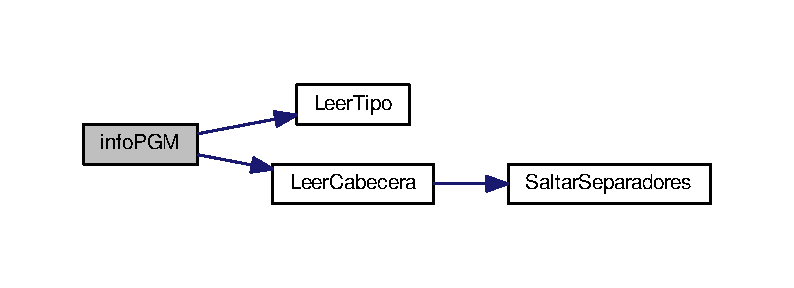
\includegraphics[width=350pt]{pgm_8h_a85c7f15bdcdee461eba76965aaccb910_cgraph}
\end{center}
\end{figure}




Gráfico de llamadas a esta función\+:
\nopagebreak
\begin{figure}[H]
\begin{center}
\leavevmode
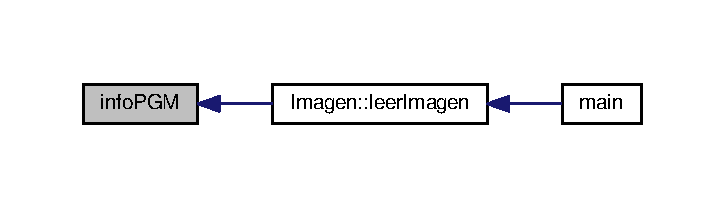
\includegraphics[width=348pt]{pgm_8h_a85c7f15bdcdee461eba76965aaccb910_icgraph}
\end{center}
\end{figure}


\hypertarget{pgm_8h_a3d11aef73fef65e3ba31446f8fc20595}{}\index{pgm.\+h@{pgm.\+h}!leer\+P\+G\+M\+Binario@{leer\+P\+G\+M\+Binario}}
\index{leer\+P\+G\+M\+Binario@{leer\+P\+G\+M\+Binario}!pgm.\+h@{pgm.\+h}}
\subsubsection[{leer\+P\+G\+M\+Binario(const char nombre[], unsigned char datos[], int \&filas, int \&columnas)}]{\setlength{\rightskip}{0pt plus 5cm}bool leer\+P\+G\+M\+Binario (
\begin{DoxyParamCaption}
\item[{const char}]{nombre\mbox{[}$\,$\mbox{]}, }
\item[{unsigned char}]{datos\mbox{[}$\,$\mbox{]}, }
\item[{int \&}]{filas, }
\item[{int \&}]{columnas}
\end{DoxyParamCaption}
)}\label{pgm_8h_a3d11aef73fef65e3ba31446f8fc20595}


Lee una imagen de tipo P\+G\+M binario. 


\begin{DoxyParams}{Parámetros}
{\em nombre} & nombre del archivo a leer \\
\hline
{\em filas} & Parámetro de salida con las filas de la imagen. \\
\hline
{\em columnas} & Parámetro de salida con las columnas de la imagen. \\
\hline
{\em datos} & vector para obtener el valor de cada uno de los píxeles desde la esquina superior izqda a la inferior dcha. \\
\hline
\end{DoxyParams}

\begin{DoxyRetVals}{Valores devueltos}
{\em true} & si ha tenido éxito en la lectura. \\
\hline
{\em false} & si se ha producido algún error en la lectura. \\
\hline
\end{DoxyRetVals}
\begin{DoxyPrecond}{Precondición}
datos debe tener tamaño suficiente para almacenar {\itshape filas} x {\itshape columnas} bytes de datos de la imagen. 
\end{DoxyPrecond}


Gráfico de llamadas para esta función\+:
\nopagebreak
\begin{figure}[H]
\begin{center}
\leavevmode
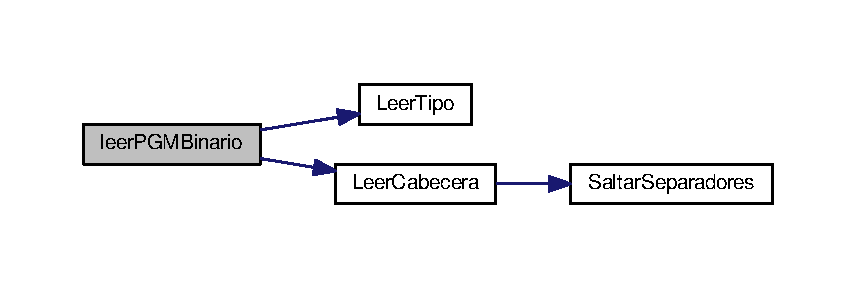
\includegraphics[width=350pt]{pgm_8h_a3d11aef73fef65e3ba31446f8fc20595_cgraph}
\end{center}
\end{figure}




Gráfico de llamadas a esta función\+:
\nopagebreak
\begin{figure}[H]
\begin{center}
\leavevmode
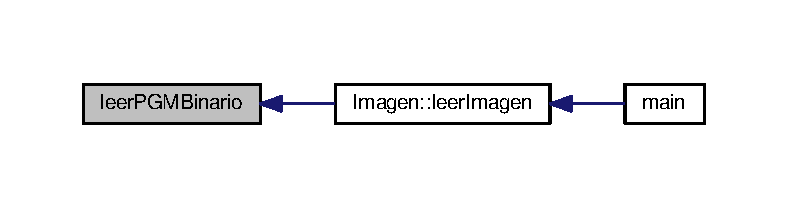
\includegraphics[width=350pt]{pgm_8h_a3d11aef73fef65e3ba31446f8fc20595_icgraph}
\end{center}
\end{figure}


\hypertarget{pgm_8h_ad0376e7bb607f570d680118ef291ee3d}{}\index{pgm.\+h@{pgm.\+h}!leer\+P\+G\+M\+Texto@{leer\+P\+G\+M\+Texto}}
\index{leer\+P\+G\+M\+Texto@{leer\+P\+G\+M\+Texto}!pgm.\+h@{pgm.\+h}}
\subsubsection[{leer\+P\+G\+M\+Texto(const char nombre[], unsigned char datos[], int \&filas, int \&columnas)}]{\setlength{\rightskip}{0pt plus 5cm}bool leer\+P\+G\+M\+Texto (
\begin{DoxyParamCaption}
\item[{const char}]{nombre\mbox{[}$\,$\mbox{]}, }
\item[{unsigned char}]{datos\mbox{[}$\,$\mbox{]}, }
\item[{int \&}]{filas, }
\item[{int \&}]{columnas}
\end{DoxyParamCaption}
)}\label{pgm_8h_ad0376e7bb607f570d680118ef291ee3d}


Gráfico de llamadas para esta función\+:
\nopagebreak
\begin{figure}[H]
\begin{center}
\leavevmode
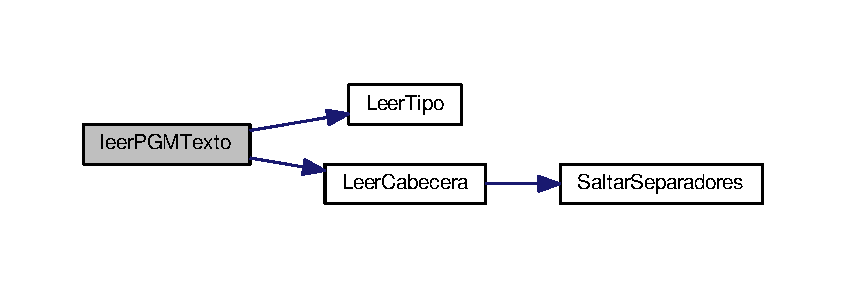
\includegraphics[width=350pt]{pgm_8h_ad0376e7bb607f570d680118ef291ee3d_cgraph}
\end{center}
\end{figure}




Gráfico de llamadas a esta función\+:
\nopagebreak
\begin{figure}[H]
\begin{center}
\leavevmode
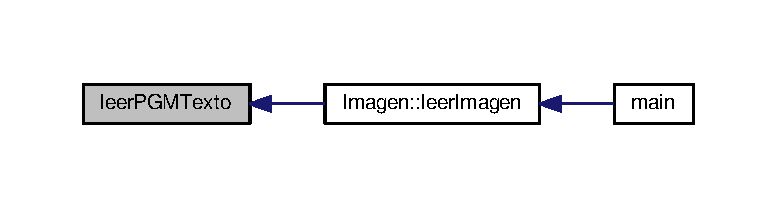
\includegraphics[width=350pt]{pgm_8h_ad0376e7bb607f570d680118ef291ee3d_icgraph}
\end{center}
\end{figure}



\hypertarget{arte_a_s_c_i_i_8cpp}{}\section{Referencia del Archivo src/arte\+A\+S\+C\+I\+I.cpp}
\label{arte_a_s_c_i_i_8cpp}\index{src/arte\+A\+S\+C\+I\+I.\+cpp@{src/arte\+A\+S\+C\+I\+I.\+cpp}}
{\ttfamily \#include $<$iostream$>$}\\*
{\ttfamily \#include $<$fstream$>$}\\*
{\ttfamily \#include $<$string$>$}\\*
{\ttfamily \#include $<$stdio.\+h$>$}\\*
{\ttfamily \#include $<$imagen.\+h$>$}\\*
{\ttfamily \#include $<$stdlib.\+h$>$}\\*
{\ttfamily \#include $<$cstring$>$}\\*
Dependencia gráfica adjunta para arte\+A\+S\+C\+I\+I.\+cpp\+:
\nopagebreak
\begin{figure}[H]
\begin{center}
\leavevmode
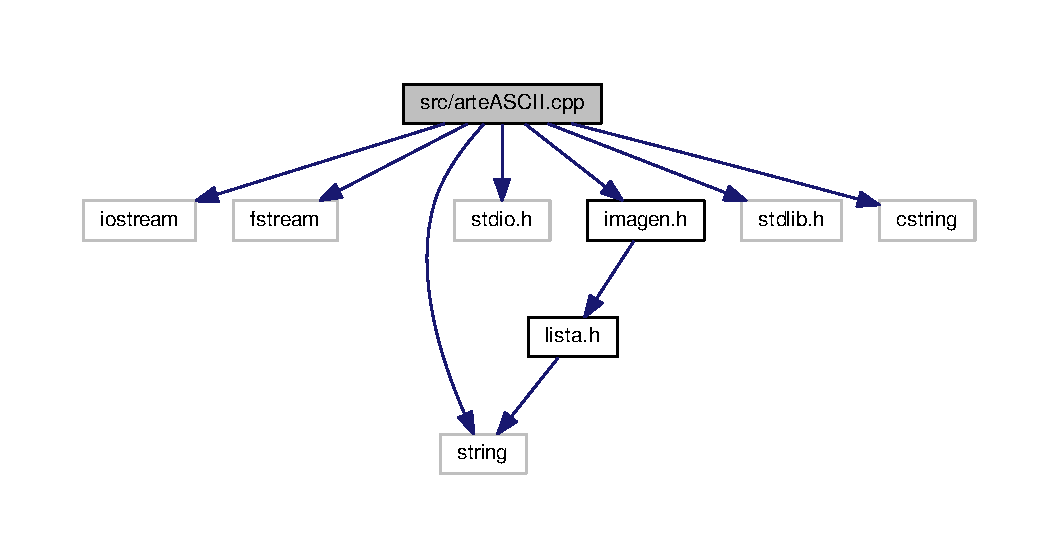
\includegraphics[width=350pt]{arte_a_s_c_i_i_8cpp__incl}
\end{center}
\end{figure}
\subsection*{Funciones}
\begin{DoxyCompactItemize}
\item 
int \hyperlink{arte_a_s_c_i_i_8cpp_ae66f6b31b5ad750f1fe042a706a4e3d4}{main} ()
\end{DoxyCompactItemize}


\subsection{Documentación de las funciones}
\hypertarget{arte_a_s_c_i_i_8cpp_ae66f6b31b5ad750f1fe042a706a4e3d4}{}\index{arte\+A\+S\+C\+I\+I.\+cpp@{arte\+A\+S\+C\+I\+I.\+cpp}!main@{main}}
\index{main@{main}!arte\+A\+S\+C\+I\+I.\+cpp@{arte\+A\+S\+C\+I\+I.\+cpp}}
\subsubsection[{main()}]{\setlength{\rightskip}{0pt plus 5cm}int main (
\begin{DoxyParamCaption}
{}
\end{DoxyParamCaption}
)}\label{arte_a_s_c_i_i_8cpp_ae66f6b31b5ad750f1fe042a706a4e3d4}


Gráfico de llamadas para esta función\+:
\nopagebreak
\begin{figure}[H]
\begin{center}
\leavevmode
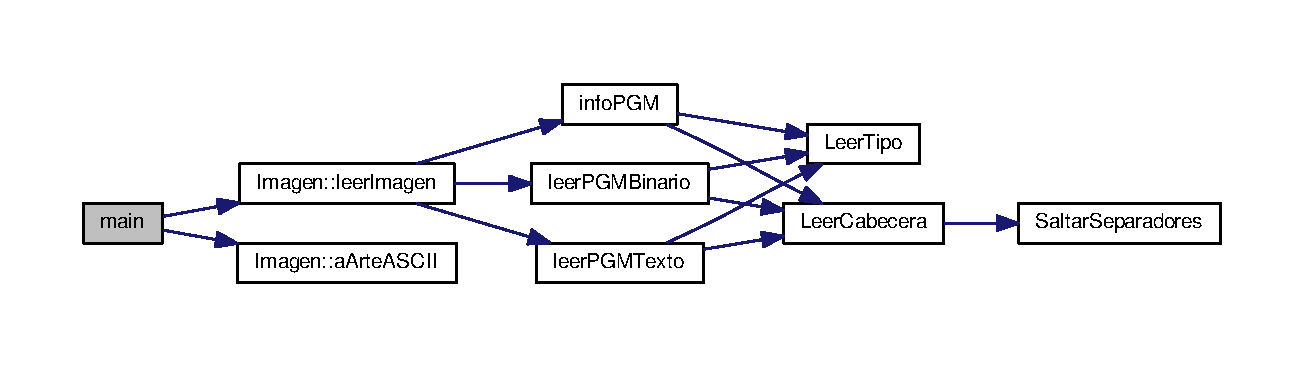
\includegraphics[width=350pt]{arte_a_s_c_i_i_8cpp_ae66f6b31b5ad750f1fe042a706a4e3d4_cgraph}
\end{center}
\end{figure}



\hypertarget{arte_a_s_c_i_i2_8cpp}{}\section{Referencia del Archivo src/arte\+A\+S\+C\+I\+I2.cpp}
\label{arte_a_s_c_i_i2_8cpp}\index{src/arte\+A\+S\+C\+I\+I2.\+cpp@{src/arte\+A\+S\+C\+I\+I2.\+cpp}}
{\ttfamily \#include $<$iostream$>$}\\*
{\ttfamily \#include $<$fstream$>$}\\*
{\ttfamily \#include $<$cstring$>$}\\*
{\ttfamily \#include \char`\"{}imagen.\+h\char`\"{}}\\*
{\ttfamily \#include \char`\"{}lista.\+h\char`\"{}}\\*
Dependencia gráfica adjunta para arte\+A\+S\+C\+I\+I2.\+cpp\+:
\nopagebreak
\begin{figure}[H]
\begin{center}
\leavevmode
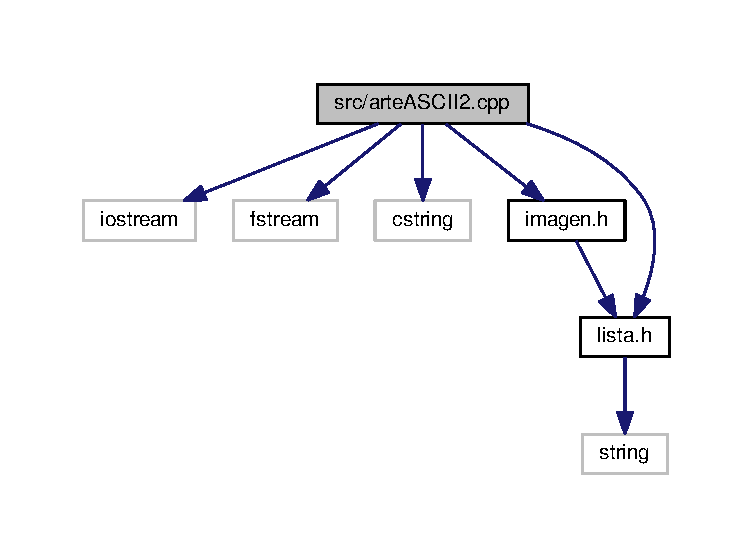
\includegraphics[width=350pt]{arte_a_s_c_i_i2_8cpp__incl}
\end{center}
\end{figure}
\subsection*{Funciones}
\begin{DoxyCompactItemize}
\item 
int \hyperlink{arte_a_s_c_i_i2_8cpp_a0ddf1224851353fc92bfbff6f499fa97}{main} (int argc, char $\ast$argv\mbox{[}$\,$\mbox{]})
\end{DoxyCompactItemize}


\subsection{Documentación de las funciones}
\hypertarget{arte_a_s_c_i_i2_8cpp_a0ddf1224851353fc92bfbff6f499fa97}{}\index{arte\+A\+S\+C\+I\+I2.\+cpp@{arte\+A\+S\+C\+I\+I2.\+cpp}!main@{main}}
\index{main@{main}!arte\+A\+S\+C\+I\+I2.\+cpp@{arte\+A\+S\+C\+I\+I2.\+cpp}}
\subsubsection[{main(int argc, char $\ast$argv[])}]{\setlength{\rightskip}{0pt plus 5cm}int main (
\begin{DoxyParamCaption}
\item[{int}]{argc, }
\item[{char $\ast$}]{argv\mbox{[}$\,$\mbox{]}}
\end{DoxyParamCaption}
)}\label{arte_a_s_c_i_i2_8cpp_a0ddf1224851353fc92bfbff6f499fa97}


Gráfico de llamadas para esta función\+:
\nopagebreak
\begin{figure}[H]
\begin{center}
\leavevmode
\includegraphics[width=350pt]{arte_a_s_c_i_i2_8cpp_a0ddf1224851353fc92bfbff6f499fa97_cgraph}
\end{center}
\end{figure}



\hypertarget{byte_8cpp}{}\section{Referencia del Archivo src/byte.cpp}
\label{byte_8cpp}\index{src/byte.\+cpp@{src/byte.\+cpp}}
{\ttfamily \#include \char`\"{}byte.\+h\char`\"{}}\\*
Dependencia gráfica adjunta para byte.\+cpp\+:
\nopagebreak
\begin{figure}[H]
\begin{center}
\leavevmode
\includegraphics[width=194pt]{byte_8cpp__incl}
\end{center}
\end{figure}
\subsection*{Namespaces}
\begin{DoxyCompactItemize}
\item 
 \hyperlink{namespacebytaso}{bytaso}
\end{DoxyCompactItemize}
\subsection*{Funciones}
\begin{DoxyCompactItemize}
\item 
void \hyperlink{namespacebytaso_ae98a18093e63134e5f1ddec44973c6ec}{bytaso\+::on} (\hyperlink{imagen_8h_a0c8186d9b9b7880309c27230bbb5e69d}{byte} \&b, int pos)
\begin{DoxyCompactList}\small\item\em enciende el bit {\ttfamily pos} del {\ttfamily byte} {\ttfamily b} \end{DoxyCompactList}\item 
void \hyperlink{namespacebytaso_a477a14f602dcc9264dbb6f874d170834}{bytaso\+::off} (\hyperlink{imagen_8h_a0c8186d9b9b7880309c27230bbb5e69d}{byte} \&b, int pos)
\begin{DoxyCompactList}\small\item\em apaga el bit {\ttfamily pos} del {\ttfamily byte} {\ttfamily b} \end{DoxyCompactList}\item 
bool \hyperlink{namespacebytaso_ad231ba96547f99130292527f5d65694b}{bytaso\+::get} (\hyperlink{imagen_8h_a0c8186d9b9b7880309c27230bbb5e69d}{byte} b, int pos)
\begin{DoxyCompactList}\small\item\em devuelve el estado del bit (encendido = true, apagado = false) en la posici�n {\ttfamily pos} \end{DoxyCompactList}\item 
string \hyperlink{namespacebytaso_a01303edb3c075bbf9f10324914352a50}{bytaso\+::byte\+To\+String} (\hyperlink{imagen_8h_a0c8186d9b9b7880309c27230bbb5e69d}{byte} b)
\begin{DoxyCompactList}\small\item\em Muestra por la salida est�ndar una secuencia de 0s y 1s correspondiente al estado de cada bit. \end{DoxyCompactList}\item 
void \hyperlink{namespacebytaso_a29bc6fb2d3ca8a24ee9a8fc044aed54a}{bytaso\+::apagar} (\hyperlink{imagen_8h_a0c8186d9b9b7880309c27230bbb5e69d}{byte} \&b)
\begin{DoxyCompactList}\small\item\em apaga todos los bits \end{DoxyCompactList}\item 
void \hyperlink{namespacebytaso_a5e016205a37415abe06efd845593bc2a}{bytaso\+::encender} (\hyperlink{imagen_8h_a0c8186d9b9b7880309c27230bbb5e69d}{byte} \&b)
\begin{DoxyCompactList}\small\item\em enciende todos los bits \end{DoxyCompactList}\item 
void \hyperlink{namespacebytaso_ae93ec524c1a740b4144a2ec249d07446}{bytaso\+::asignar} (\hyperlink{imagen_8h_a0c8186d9b9b7880309c27230bbb5e69d}{byte} \&b, const bool v\mbox{[}$\,$\mbox{]})
\begin{DoxyCompactList}\small\item\em enciende los bits seg�n la configuraci�n de {\ttfamily v} \end{DoxyCompactList}\item 
void \hyperlink{namespacebytaso_aca892e499e255f8b8a967b67cd164a75}{bytaso\+::volcar} (\hyperlink{imagen_8h_a0c8186d9b9b7880309c27230bbb5e69d}{byte} b, bool v\mbox{[}$\,$\mbox{]})
\begin{DoxyCompactList}\small\item\em recupera la configuraci�n de todos los bit \end{DoxyCompactList}\item 
void \hyperlink{namespacebytaso_a76ad23326440e16a7b419ee7a14ee287}{bytaso\+::encendidos} (\hyperlink{imagen_8h_a0c8186d9b9b7880309c27230bbb5e69d}{byte} b, int posic\mbox{[}$\,$\mbox{]}, int \&cuantos)
\begin{DoxyCompactList}\small\item\em devuelve las posiciones de los bits encendidos \end{DoxyCompactList}\end{DoxyCompactItemize}

\hypertarget{imagen_8cpp}{}\section{Referencia del Archivo src/imagen.cpp}
\label{imagen_8cpp}\index{src/imagen.\+cpp@{src/imagen.\+cpp}}
{\ttfamily \#include \char`\"{}imagen.\+h\char`\"{}}\\*
{\ttfamily \#include \char`\"{}lista.\+h\char`\"{}}\\*
{\ttfamily \#include \char`\"{}pgm.\+h\char`\"{}}\\*
{\ttfamily \#include \char`\"{}byte.\+h\char`\"{}}\\*
{\ttfamily \#include $<$stdlib.\+h$>$}\\*
{\ttfamily \#include $<$stdio.\+h$>$}\\*
{\ttfamily \#include $<$iostream$>$}\\*
{\ttfamily \#include $<$fstream$>$}\\*
{\ttfamily \#include $<$cstring$>$}\\*
{\ttfamily \#include $<$string.\+h$>$}\\*
Dependencia gráfica adjunta para imagen.\+cpp\+:
\nopagebreak
\begin{figure}[H]
\begin{center}
\leavevmode
\includegraphics[width=350pt]{imagen_8cpp__incl}
\end{center}
\end{figure}

\hypertarget{lista_8cpp}{}\section{Referencia del Archivo src/lista.cpp}
\label{lista_8cpp}\index{src/lista.\+cpp@{src/lista.\+cpp}}
{\ttfamily \#include $<$string$>$}\\*
{\ttfamily \#include $<$fstream$>$}\\*
{\ttfamily \#include $<$iostream$>$}\\*
{\ttfamily \#include \char`\"{}lista.\+h\char`\"{}}\\*
Dependencia gráfica adjunta para lista.\+cpp\+:
\nopagebreak
\begin{figure}[H]
\begin{center}
\leavevmode
\includegraphics[width=276pt]{lista_8cpp__incl}
\end{center}
\end{figure}

\hypertarget{pgm_8cpp}{}\section{Referencia del Archivo src/pgm.cpp}
\label{pgm_8cpp}\index{src/pgm.\+cpp@{src/pgm.\+cpp}}


Fichero con las definiciones para la E/\+S de imágenes P\+G\+M.  


{\ttfamily \#include $<$fstream$>$}\\*
{\ttfamily \#include $<$string$>$}\\*
{\ttfamily \#include \char`\"{}pgm.\+h\char`\"{}}\\*
Dependencia gráfica adjunta para pgm.\+cpp\+:
\nopagebreak
\begin{figure}[H]
\begin{center}
\leavevmode
\includegraphics[width=252pt]{pgm_8cpp__incl}
\end{center}
\end{figure}
\subsection*{Funciones}
\begin{DoxyCompactItemize}
\item 
\hyperlink{pgm_8h_a8914f6544a484741b05c092d9e7522ed}{Tipo\+Imagen} \hyperlink{pgm_8cpp_a16834dd3756f7baf1e5ef710ad7b0e3b}{Leer\+Tipo} (ifstream \&f)
\item 
char \hyperlink{pgm_8cpp_ab090ad072f47dc1ffcfcb900c3334936}{Saltar\+Separadores} (ifstream \&f)
\item 
bool \hyperlink{pgm_8cpp_af6fdaef0f7391aa844eea8e2f4b0f235}{Leer\+Cabecera} (ifstream \&f, int \&filas, int \&columnas)
\item 
\hyperlink{pgm_8h_a8914f6544a484741b05c092d9e7522ed}{Tipo\+Imagen} \hyperlink{pgm_8cpp_a85c7f15bdcdee461eba76965aaccb910}{info\+P\+G\+M} (const char nombre\mbox{[}$\,$\mbox{]}, int \&filas, int \&columnas)
\begin{DoxyCompactList}\small\item\em Consulta el tipo de imagen del archivo y sus dimensiones. \end{DoxyCompactList}\item 
bool \hyperlink{pgm_8cpp_a3d11aef73fef65e3ba31446f8fc20595}{leer\+P\+G\+M\+Binario} (const char nombre\mbox{[}$\,$\mbox{]}, unsigned char datos\mbox{[}$\,$\mbox{]}, int \&filas, int \&columnas)
\begin{DoxyCompactList}\small\item\em Lee una imagen de tipo P\+G\+M binario. \end{DoxyCompactList}\item 
bool \hyperlink{pgm_8cpp_a381cd69ce2e9de0b0e3b12131a397121}{escribir\+P\+G\+M\+Binario} (const char nombre\mbox{[}$\,$\mbox{]}, const unsigned char datos\mbox{[}$\,$\mbox{]}, int filas, int columnas)
\begin{DoxyCompactList}\small\item\em Escribe una imagen de tipo P\+G\+M binario. \end{DoxyCompactList}\item 
bool \hyperlink{pgm_8cpp_ad0376e7bb607f570d680118ef291ee3d}{leer\+P\+G\+M\+Texto} (const char nombre\mbox{[}$\,$\mbox{]}, unsigned char datos\mbox{[}$\,$\mbox{]}, int \&filas, int \&columnas)
\item 
bool \hyperlink{pgm_8cpp_a0ecaed351740580902d90a4c496a0e3b}{escribir\+P\+G\+M\+Texto} (const char nombre\mbox{[}$\,$\mbox{]}, const unsigned char datos\mbox{[}$\,$\mbox{]}, int filas, int columnas)
\end{DoxyCompactItemize}


\subsection{Descripción detallada}
Fichero con las definiciones para la E/\+S de imágenes P\+G\+M. 

Permite la E/\+S de archivos de tipos P\+G\+M 

\subsection{Documentación de las funciones}
\hypertarget{pgm_8cpp_a381cd69ce2e9de0b0e3b12131a397121}{}\index{pgm.\+cpp@{pgm.\+cpp}!escribir\+P\+G\+M\+Binario@{escribir\+P\+G\+M\+Binario}}
\index{escribir\+P\+G\+M\+Binario@{escribir\+P\+G\+M\+Binario}!pgm.\+cpp@{pgm.\+cpp}}
\subsubsection[{escribir\+P\+G\+M\+Binario(const char nombre[], const unsigned char datos[], int filas, int columnas)}]{\setlength{\rightskip}{0pt plus 5cm}bool escribir\+P\+G\+M\+Binario (
\begin{DoxyParamCaption}
\item[{const char}]{nombre\mbox{[}$\,$\mbox{]}, }
\item[{const unsigned char}]{datos\mbox{[}$\,$\mbox{]}, }
\item[{int}]{filas, }
\item[{int}]{columnas}
\end{DoxyParamCaption}
)}\label{pgm_8cpp_a381cd69ce2e9de0b0e3b12131a397121}


Escribe una imagen de tipo P\+G\+M binario. 


\begin{DoxyParams}{Parámetros}
{\em nombre} & nombre del archivo a escribir \\
\hline
{\em datos} & vector con {\itshape filas} x {\itshape columnas} bytes que corresponden a los valores de los píxeles de la imagen de grises. \\
\hline
{\em filas} & número de filas de la imagen \\
\hline
{\em columnas} & número de columnas de la imagen \\
\hline
\end{DoxyParams}

\begin{DoxyRetVals}{Valores devueltos}
{\em true} & si ha tenido éxito en la escritura. \\
\hline
{\em false} & si se ha producido algún error en la escritura. \\
\hline
\end{DoxyRetVals}


Gráfico de llamadas a esta función\+:
\nopagebreak
\begin{figure}[H]
\begin{center}
\leavevmode
\includegraphics[width=350pt]{pgm_8cpp_a381cd69ce2e9de0b0e3b12131a397121_icgraph}
\end{center}
\end{figure}


\hypertarget{pgm_8cpp_a0ecaed351740580902d90a4c496a0e3b}{}\index{pgm.\+cpp@{pgm.\+cpp}!escribir\+P\+G\+M\+Texto@{escribir\+P\+G\+M\+Texto}}
\index{escribir\+P\+G\+M\+Texto@{escribir\+P\+G\+M\+Texto}!pgm.\+cpp@{pgm.\+cpp}}
\subsubsection[{escribir\+P\+G\+M\+Texto(const char nombre[], const unsigned char datos[], int filas, int columnas)}]{\setlength{\rightskip}{0pt plus 5cm}bool escribir\+P\+G\+M\+Texto (
\begin{DoxyParamCaption}
\item[{const char}]{nombre\mbox{[}$\,$\mbox{]}, }
\item[{const unsigned char}]{datos\mbox{[}$\,$\mbox{]}, }
\item[{int}]{filas, }
\item[{int}]{columnas}
\end{DoxyParamCaption}
)}\label{pgm_8cpp_a0ecaed351740580902d90a4c496a0e3b}


Gráfico de llamadas a esta función\+:
\nopagebreak
\begin{figure}[H]
\begin{center}
\leavevmode
\includegraphics[width=350pt]{pgm_8cpp_a0ecaed351740580902d90a4c496a0e3b_icgraph}
\end{center}
\end{figure}


\hypertarget{pgm_8cpp_a85c7f15bdcdee461eba76965aaccb910}{}\index{pgm.\+cpp@{pgm.\+cpp}!info\+P\+G\+M@{info\+P\+G\+M}}
\index{info\+P\+G\+M@{info\+P\+G\+M}!pgm.\+cpp@{pgm.\+cpp}}
\subsubsection[{info\+P\+G\+M(const char nombre[], int \&filas, int \&columnas)}]{\setlength{\rightskip}{0pt plus 5cm}{\bf Tipo\+Imagen} info\+P\+G\+M (
\begin{DoxyParamCaption}
\item[{const char}]{nombre\mbox{[}$\,$\mbox{]}, }
\item[{int \&}]{filas, }
\item[{int \&}]{columnas}
\end{DoxyParamCaption}
)}\label{pgm_8cpp_a85c7f15bdcdee461eba76965aaccb910}


Consulta el tipo de imagen del archivo y sus dimensiones. 


\begin{DoxyParams}{Parámetros}
{\em nombre} & indica el nombre del archivo de disco a consultar \\
\hline
{\em filas} & Parámetro de salida con las filas de la imagen. \\
\hline
{\em columnas} & Parámetro de salida con las columnas de la imagen. \\
\hline
\end{DoxyParams}
\begin{DoxyReturn}{Devuelve}
Devuelve el tipo de la imagen en el archivo
\end{DoxyReturn}
\begin{DoxySeeAlso}{Ver también}
\hyperlink{pgm_8h_a8914f6544a484741b05c092d9e7522ed}{Tipo\+Imagen} 
\end{DoxySeeAlso}


Gráfico de llamadas para esta función\+:
\nopagebreak
\begin{figure}[H]
\begin{center}
\leavevmode
\includegraphics[width=350pt]{pgm_8cpp_a85c7f15bdcdee461eba76965aaccb910_cgraph}
\end{center}
\end{figure}




Gráfico de llamadas a esta función\+:
\nopagebreak
\begin{figure}[H]
\begin{center}
\leavevmode
\includegraphics[width=348pt]{pgm_8cpp_a85c7f15bdcdee461eba76965aaccb910_icgraph}
\end{center}
\end{figure}


\hypertarget{pgm_8cpp_af6fdaef0f7391aa844eea8e2f4b0f235}{}\index{pgm.\+cpp@{pgm.\+cpp}!Leer\+Cabecera@{Leer\+Cabecera}}
\index{Leer\+Cabecera@{Leer\+Cabecera}!pgm.\+cpp@{pgm.\+cpp}}
\subsubsection[{Leer\+Cabecera(ifstream \&f, int \&filas, int \&columnas)}]{\setlength{\rightskip}{0pt plus 5cm}bool Leer\+Cabecera (
\begin{DoxyParamCaption}
\item[{ifstream \&}]{f, }
\item[{int \&}]{filas, }
\item[{int \&}]{columnas}
\end{DoxyParamCaption}
)}\label{pgm_8cpp_af6fdaef0f7391aa844eea8e2f4b0f235}


Gráfico de llamadas para esta función\+:
\nopagebreak
\begin{figure}[H]
\begin{center}
\leavevmode
\includegraphics[width=290pt]{pgm_8cpp_af6fdaef0f7391aa844eea8e2f4b0f235_cgraph}
\end{center}
\end{figure}




Gráfico de llamadas a esta función\+:
\nopagebreak
\begin{figure}[H]
\begin{center}
\leavevmode
\includegraphics[width=350pt]{pgm_8cpp_af6fdaef0f7391aa844eea8e2f4b0f235_icgraph}
\end{center}
\end{figure}


\hypertarget{pgm_8cpp_a3d11aef73fef65e3ba31446f8fc20595}{}\index{pgm.\+cpp@{pgm.\+cpp}!leer\+P\+G\+M\+Binario@{leer\+P\+G\+M\+Binario}}
\index{leer\+P\+G\+M\+Binario@{leer\+P\+G\+M\+Binario}!pgm.\+cpp@{pgm.\+cpp}}
\subsubsection[{leer\+P\+G\+M\+Binario(const char nombre[], unsigned char datos[], int \&filas, int \&columnas)}]{\setlength{\rightskip}{0pt plus 5cm}bool leer\+P\+G\+M\+Binario (
\begin{DoxyParamCaption}
\item[{const char}]{nombre\mbox{[}$\,$\mbox{]}, }
\item[{unsigned char}]{datos\mbox{[}$\,$\mbox{]}, }
\item[{int \&}]{filas, }
\item[{int \&}]{columnas}
\end{DoxyParamCaption}
)}\label{pgm_8cpp_a3d11aef73fef65e3ba31446f8fc20595}


Lee una imagen de tipo P\+G\+M binario. 


\begin{DoxyParams}{Parámetros}
{\em nombre} & nombre del archivo a leer \\
\hline
{\em filas} & Parámetro de salida con las filas de la imagen. \\
\hline
{\em columnas} & Parámetro de salida con las columnas de la imagen. \\
\hline
{\em datos} & vector para obtener el valor de cada uno de los píxeles desde la esquina superior izqda a la inferior dcha. \\
\hline
\end{DoxyParams}

\begin{DoxyRetVals}{Valores devueltos}
{\em true} & si ha tenido éxito en la lectura. \\
\hline
{\em false} & si se ha producido algún error en la lectura. \\
\hline
\end{DoxyRetVals}
\begin{DoxyPrecond}{Precondición}
datos debe tener tamaño suficiente para almacenar {\itshape filas} x {\itshape columnas} bytes de datos de la imagen. 
\end{DoxyPrecond}


Gráfico de llamadas para esta función\+:
\nopagebreak
\begin{figure}[H]
\begin{center}
\leavevmode
\includegraphics[width=350pt]{pgm_8cpp_a3d11aef73fef65e3ba31446f8fc20595_cgraph}
\end{center}
\end{figure}




Gráfico de llamadas a esta función\+:
\nopagebreak
\begin{figure}[H]
\begin{center}
\leavevmode
\includegraphics[width=350pt]{pgm_8cpp_a3d11aef73fef65e3ba31446f8fc20595_icgraph}
\end{center}
\end{figure}


\hypertarget{pgm_8cpp_ad0376e7bb607f570d680118ef291ee3d}{}\index{pgm.\+cpp@{pgm.\+cpp}!leer\+P\+G\+M\+Texto@{leer\+P\+G\+M\+Texto}}
\index{leer\+P\+G\+M\+Texto@{leer\+P\+G\+M\+Texto}!pgm.\+cpp@{pgm.\+cpp}}
\subsubsection[{leer\+P\+G\+M\+Texto(const char nombre[], unsigned char datos[], int \&filas, int \&columnas)}]{\setlength{\rightskip}{0pt plus 5cm}bool leer\+P\+G\+M\+Texto (
\begin{DoxyParamCaption}
\item[{const char}]{nombre\mbox{[}$\,$\mbox{]}, }
\item[{unsigned char}]{datos\mbox{[}$\,$\mbox{]}, }
\item[{int \&}]{filas, }
\item[{int \&}]{columnas}
\end{DoxyParamCaption}
)}\label{pgm_8cpp_ad0376e7bb607f570d680118ef291ee3d}


Gráfico de llamadas para esta función\+:
\nopagebreak
\begin{figure}[H]
\begin{center}
\leavevmode
\includegraphics[width=350pt]{pgm_8cpp_ad0376e7bb607f570d680118ef291ee3d_cgraph}
\end{center}
\end{figure}




Gráfico de llamadas a esta función\+:
\nopagebreak
\begin{figure}[H]
\begin{center}
\leavevmode
\includegraphics[width=350pt]{pgm_8cpp_ad0376e7bb607f570d680118ef291ee3d_icgraph}
\end{center}
\end{figure}


\hypertarget{pgm_8cpp_a16834dd3756f7baf1e5ef710ad7b0e3b}{}\index{pgm.\+cpp@{pgm.\+cpp}!Leer\+Tipo@{Leer\+Tipo}}
\index{Leer\+Tipo@{Leer\+Tipo}!pgm.\+cpp@{pgm.\+cpp}}
\subsubsection[{Leer\+Tipo(ifstream \&f)}]{\setlength{\rightskip}{0pt plus 5cm}{\bf Tipo\+Imagen} Leer\+Tipo (
\begin{DoxyParamCaption}
\item[{ifstream \&}]{f}
\end{DoxyParamCaption}
)}\label{pgm_8cpp_a16834dd3756f7baf1e5ef710ad7b0e3b}


Gráfico de llamadas a esta función\+:
\nopagebreak
\begin{figure}[H]
\begin{center}
\leavevmode
\includegraphics[width=350pt]{pgm_8cpp_a16834dd3756f7baf1e5ef710ad7b0e3b_icgraph}
\end{center}
\end{figure}


\hypertarget{pgm_8cpp_ab090ad072f47dc1ffcfcb900c3334936}{}\index{pgm.\+cpp@{pgm.\+cpp}!Saltar\+Separadores@{Saltar\+Separadores}}
\index{Saltar\+Separadores@{Saltar\+Separadores}!pgm.\+cpp@{pgm.\+cpp}}
\subsubsection[{Saltar\+Separadores(ifstream \&f)}]{\setlength{\rightskip}{0pt plus 5cm}char Saltar\+Separadores (
\begin{DoxyParamCaption}
\item[{ifstream \&}]{f}
\end{DoxyParamCaption}
)}\label{pgm_8cpp_ab090ad072f47dc1ffcfcb900c3334936}


Gráfico de llamadas a esta función\+:
\nopagebreak
\begin{figure}[H]
\begin{center}
\leavevmode
\includegraphics[width=350pt]{pgm_8cpp_ab090ad072f47dc1ffcfcb900c3334936_icgraph}
\end{center}
\end{figure}



\hypertarget{suma_8cpp}{}\section{Referencia del Archivo src/suma.cpp}
\label{suma_8cpp}\index{src/suma.\+cpp@{src/suma.\+cpp}}
{\ttfamily \#include $<$iostream$>$}\\*
{\ttfamily \#include $<$imagen.\+h$>$}\\*
Dependencia gráfica adjunta para suma.\+cpp\+:
\nopagebreak
\begin{figure}[H]
\begin{center}
\leavevmode
\includegraphics[width=208pt]{suma_8cpp__incl}
\end{center}
\end{figure}
\subsection*{Funciones}
\begin{DoxyCompactItemize}
\item 
int \hyperlink{suma_8cpp_a0ddf1224851353fc92bfbff6f499fa97}{main} (int argc, char $\ast$argv\mbox{[}$\,$\mbox{]})
\end{DoxyCompactItemize}


\subsection{Documentación de las funciones}
\hypertarget{suma_8cpp_a0ddf1224851353fc92bfbff6f499fa97}{}\index{suma.\+cpp@{suma.\+cpp}!main@{main}}
\index{main@{main}!suma.\+cpp@{suma.\+cpp}}
\subsubsection[{main(int argc, char $\ast$argv[])}]{\setlength{\rightskip}{0pt plus 5cm}int main (
\begin{DoxyParamCaption}
\item[{int}]{argc, }
\item[{char $\ast$}]{argv\mbox{[}$\,$\mbox{]}}
\end{DoxyParamCaption}
)}\label{suma_8cpp_a0ddf1224851353fc92bfbff6f499fa97}


Gráfico de llamadas para esta función\+:
\nopagebreak
\begin{figure}[H]
\begin{center}
\leavevmode
\includegraphics[width=350pt]{suma_8cpp_a0ddf1224851353fc92bfbff6f499fa97_cgraph}
\end{center}
\end{figure}



\hypertarget{testarte_a_s_c_i_i_8cpp}{}\section{Referencia del Archivo src/testarte\+A\+S\+C\+I\+I.cpp}
\label{testarte_a_s_c_i_i_8cpp}\index{src/testarte\+A\+S\+C\+I\+I.\+cpp@{src/testarte\+A\+S\+C\+I\+I.\+cpp}}
{\ttfamily \#include $<$iostream$>$}\\*
{\ttfamily \#include $<$imagen.\+h$>$}\\*
Dependencia gráfica adjunta para testarte\+A\+S\+C\+I\+I.\+cpp\+:
\nopagebreak
\begin{figure}[H]
\begin{center}
\leavevmode
\includegraphics[width=208pt]{testarte_a_s_c_i_i_8cpp__incl}
\end{center}
\end{figure}
\subsection*{Funciones}
\begin{DoxyCompactItemize}
\item 
int \hyperlink{testarte_a_s_c_i_i_8cpp_ae66f6b31b5ad750f1fe042a706a4e3d4}{main} ()
\end{DoxyCompactItemize}


\subsection{Documentación de las funciones}
\hypertarget{testarte_a_s_c_i_i_8cpp_ae66f6b31b5ad750f1fe042a706a4e3d4}{}\index{testarte\+A\+S\+C\+I\+I.\+cpp@{testarte\+A\+S\+C\+I\+I.\+cpp}!main@{main}}
\index{main@{main}!testarte\+A\+S\+C\+I\+I.\+cpp@{testarte\+A\+S\+C\+I\+I.\+cpp}}
\subsubsection[{main()}]{\setlength{\rightskip}{0pt plus 5cm}int main (
\begin{DoxyParamCaption}
{}
\end{DoxyParamCaption}
)}\label{testarte_a_s_c_i_i_8cpp_ae66f6b31b5ad750f1fe042a706a4e3d4}


Gráfico de llamadas para esta función\+:
\nopagebreak
\begin{figure}[H]
\begin{center}
\leavevmode
\includegraphics[width=350pt]{testarte_a_s_c_i_i_8cpp_ae66f6b31b5ad750f1fe042a706a4e3d4_cgraph}
\end{center}
\end{figure}



\hypertarget{testimagen_8cpp}{}\section{Referencia del Archivo src/testimagen.cpp}
\label{testimagen_8cpp}\index{src/testimagen.\+cpp@{src/testimagen.\+cpp}}
{\ttfamily \#include $<$iostream$>$}\\*
{\ttfamily \#include $<$imagen.\+h$>$}\\*
Dependencia gráfica adjunta para testimagen.\+cpp\+:
\nopagebreak
\begin{figure}[H]
\begin{center}
\leavevmode
\includegraphics[width=208pt]{testimagen_8cpp__incl}
\end{center}
\end{figure}
\subsection*{Funciones}
\begin{DoxyCompactItemize}
\item 
int \hyperlink{testimagen_8cpp_ae66f6b31b5ad750f1fe042a706a4e3d4}{main} ()
\end{DoxyCompactItemize}


\subsection{Documentación de las funciones}
\hypertarget{testimagen_8cpp_ae66f6b31b5ad750f1fe042a706a4e3d4}{}\index{testimagen.\+cpp@{testimagen.\+cpp}!main@{main}}
\index{main@{main}!testimagen.\+cpp@{testimagen.\+cpp}}
\subsubsection[{main()}]{\setlength{\rightskip}{0pt plus 5cm}int main (
\begin{DoxyParamCaption}
{}
\end{DoxyParamCaption}
)}\label{testimagen_8cpp_ae66f6b31b5ad750f1fe042a706a4e3d4}


Gráfico de llamadas para esta función\+:
\nopagebreak
\begin{figure}[H]
\begin{center}
\leavevmode
\includegraphics[width=350pt]{testimagen_8cpp_ae66f6b31b5ad750f1fe042a706a4e3d4_cgraph}
\end{center}
\end{figure}



\hypertarget{testplano_8cpp}{}\section{Referencia del Archivo src/testplano.cpp}
\label{testplano_8cpp}\index{src/testplano.\+cpp@{src/testplano.\+cpp}}
{\ttfamily \#include $<$iostream$>$}\\*
{\ttfamily \#include $<$imagen.\+h$>$}\\*
Dependencia gráfica adjunta para testplano.\+cpp\+:
\nopagebreak
\begin{figure}[H]
\begin{center}
\leavevmode
\includegraphics[width=208pt]{testplano_8cpp__incl}
\end{center}
\end{figure}
\subsection*{Funciones}
\begin{DoxyCompactItemize}
\item 
int \hyperlink{testplano_8cpp_ae66f6b31b5ad750f1fe042a706a4e3d4}{main} ()
\end{DoxyCompactItemize}


\subsection{Documentación de las funciones}
\hypertarget{testplano_8cpp_ae66f6b31b5ad750f1fe042a706a4e3d4}{}\index{testplano.\+cpp@{testplano.\+cpp}!main@{main}}
\index{main@{main}!testplano.\+cpp@{testplano.\+cpp}}
\subsubsection[{main()}]{\setlength{\rightskip}{0pt plus 5cm}int main (
\begin{DoxyParamCaption}
{}
\end{DoxyParamCaption}
)}\label{testplano_8cpp_ae66f6b31b5ad750f1fe042a706a4e3d4}


Gráfico de llamadas para esta función\+:
\nopagebreak
\begin{figure}[H]
\begin{center}
\leavevmode
\includegraphics[width=350pt]{testplano_8cpp_ae66f6b31b5ad750f1fe042a706a4e3d4_cgraph}
\end{center}
\end{figure}



%--- End generated contents ---

% Index
\backmatter
\newpage
\phantomsection
\clearemptydoublepage
\addcontentsline{toc}{chapter}{Índice}
\printindex

\end{document}
